\documentclass[11pt,a4paper,twoside,onecolumn,openright,final]{memoir}
\usepackage[T1]{fontenc}
\usepackage[utf8]{inputenc}
\usepackage[greek,english]{babel}
\usepackage{alphabeta}
\usepackage{graphicx}
\usepackage{array}
\graphicspath{ {figures/} }
\usepackage{epstopdf}
\usepackage{wrapfig}
\usepackage{amsmath}
\usepackage{amssymb}
\usepackage{amsthm}
\usepackage{psfrag}
\usepackage[numbers,sort&compress]{natbib}
\makeatletter\let\c@lofdepth\relax\let\c@lotdepth\relax\makeatother
\usepackage[small,bf,tight]{subfigure}
\usepackage{textcomp}
\usepackage{mathrsfs}
\usepackage{tikz}
\usepackage{pgfplots}
\pgfplotsset{compat=1.15}
\usetikzlibrary{arrows}
\usepackage{geometry}
\geometry{total={210mm,297mm},left=25mm,right=25mm,bindingoffset=0mm, top=25mm,bottom=25mm}
\usepackage[breaklinks=true,colorlinks=true,
linkcolor=blue,urlcolor=blue,citecolor=blue,% PDF VIEW
%linkcolor=black,urlcolor=black,citecolor=black,% PRINT
bookmarks=false,bookmarksopenlevel=2]{hyperref}
\usepackage{algorithm}
\usepackage{algpseudocode}
%\usepackage{dsfont}
%\usepackage{mathabx}

\OnehalfSpacing
\maxsecnumdepth{subsubsection}
\maxtocdepth{subsubsection}
\newtheorem{theorem}{Θεώρημα}
\newtheorem{lemma}{Λήμμα}
\newtheorem{remark}{Σχόλιο}
\newtheorem{example}{Παράδειγμα}
\newtheorem{definition}{Ορισμός}
\newtheorem{question}{Ερώτημα}
\renewenvironment{proof}{\emph{Απόδειξη:}}{\hfill $\blacksquare$ \\}
\renewcommand\qedsymbol{$\blacksquare$}
\addto\captiongreek{\renewcommand\proofname{Απόδειξη}}
\newcommand*{\medcap}{\mathbin{\scalebox{1}{\ensuremath{\bigcap}}}}
\newcommand\tred[1]{\textcolor[rgb]{0.98,0.00,0.00}{#1}} % for red-text





\begin{document}

%COVER PAGE%%%%%%%%%%%%%%%%%%%%%%%%%%%%%%%%%%%%%%%%%%%%%%%%%%%%%%%%%%%%%%%%%%%%%
\thispagestyle{empty}
{\centering\Large

\vspace{\fill}

{\Large Αριστοτέλειο Πανεπιστήμιο Θεσσαλονίκης\\
Τμήμα Ηλεκτρολόγων Μηχανικών και Μηχανικών Υπολογιστών}\\[0.5cm]

\begin{figure}[h]
\centerfloat%

\includegraphics[width=3.0cm]{figures/logo_auth.png}
\end{figure}
\vspace{2.0cm}

{\LARGE Γκέκας Άγγελος \; 10405 \\
Παπαδάκης Κωνσταντίνος Φώτιος \; 10371 \\
Παρασίου Δημήτριος \; 11329}

\vspace{3.5cm}


{\Huge Εργασία στο μάθημα Ηλεκτρονική 2}

\vspace{3.5cm}


\vspace{\fill}

Θεσσαλονίκη, Μάιος 2025

}


%%%%%%%%%%%%%%%%%%%%%%% ABSTRACT %%%%%%%%%%%%%%%%%%%%%%%%%%%
%%%%%%%%%%%%%%%%%%%%%%%%%%%%%%%%%%%%%%%%%%%%%%%%%%%%%%%%%%%%
\let\cleardoublepage\clearpage
\frontmatter


\renewcommand*\contentsname{Περιεχόμενα}
\tableofcontents*

\renewcommand*\listfigurename{Κατάλογος Σχημάτων}
\listoffigures*

\begin{comment}
\renewcommand*\listtablename{Κατάλογος Πινάκων}
\listoftables*
\renewcommand*\listalgorithmname{Κατάλογος Αλγορίθμων}
\listofalgorithms
\end{comment}


\renewcommand*\chaptername{Κεφάλαιο}
\renewcommand*\figurename{Σχήμα}
\floatname{algorithm}{Αλγόριθμος}
\renewcommand{\tablename}{Πίνακας}

\mainmatter

%%%%%%%%%%%%%%%%%%%%%%%% Exercise 1 %%%%%%%%%%%%%%%%%%%%%%%%
%%%%%%%%%%%%%%%%%%%%%%%%%%%%%%%%%%%%%%%%%%%%%%%%%%%%%%%%%%%%

\chapter{Εργαστηριακή Άσκηση 1}

\section{Βήμα 7}

\subsection{Ανάλυση με LT spice}

\paragraph*{} Για την χρονική ανάλυση υλοποιήθηκε το κύκλωμα του σχήματος 1-7 του φυλλαδίου, όπως φαίνεται στην εικόνα \ref{fig:ex1circuit1}.

\begin{figure}[h]
\centerfloat%
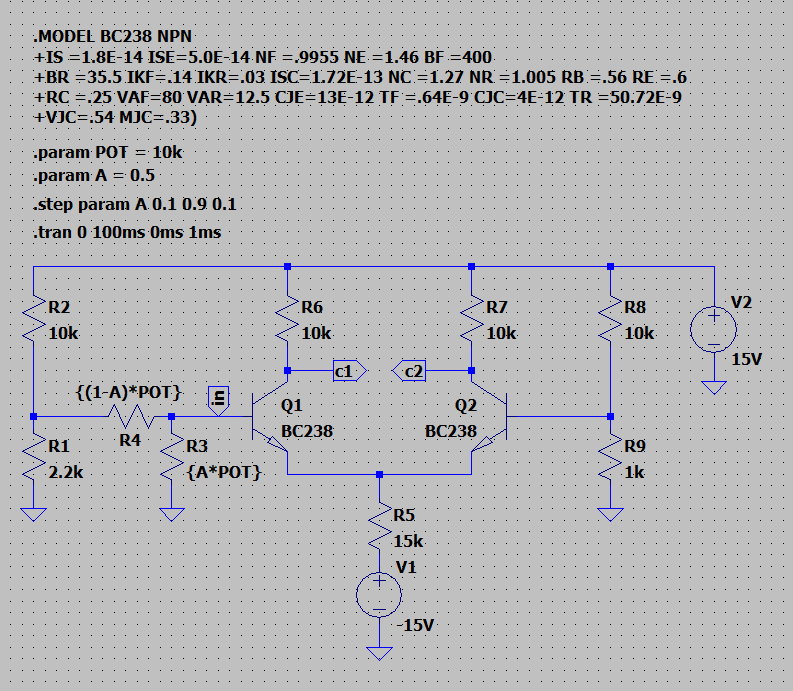
\includegraphics[width=12.0cm]{figures/exercise1circuit1.png}
\caption{Κύκλωμα Διαφορικού Ενισχυτή}\label{fig:ex1circuit1}
\end{figure}

Οι τάσεις εισόδου (in) και εξόδου (c1, c2) φαίνονται στα διαγράμματα του σχήματος \ref{fig:ex1plot1}.

\begin{figure}[h]
\centerfloat%
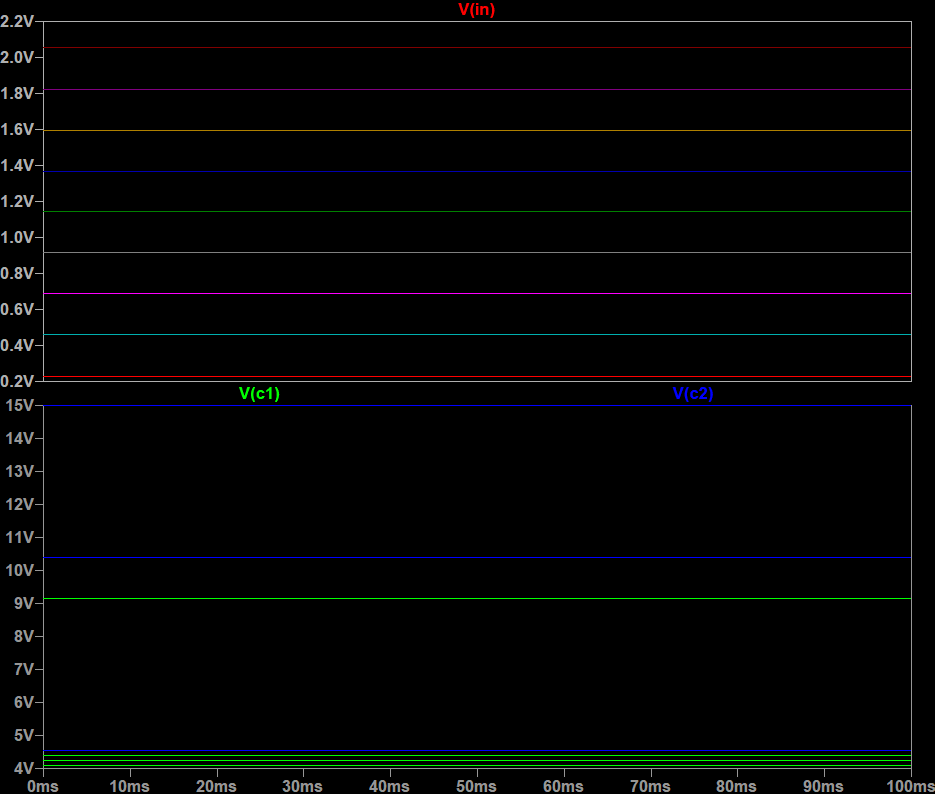
\includegraphics[width=10.0cm]{figures/exercise1plot1.png}
\caption{Είσοδος και Έξοδος Ενισχυτή με Χρονική Ανάλυση}\label{fig:ex1plot1}
\end{figure}

Για την ανάλυση DC sweep αντικαταστάθηκε ο ροοστάτης με μια πηγή τάσης, όπως φαίνεται στο σχήμα \ref{fig:ex1circuit2}.

\begin{figure}[h]
\centerfloat%
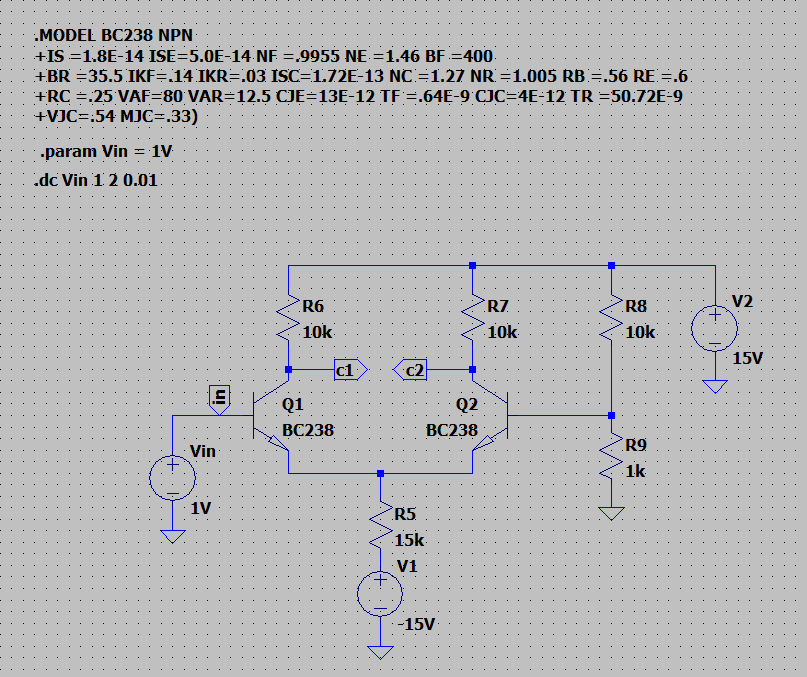
\includegraphics[width=12.0cm]{figures/exercise1circuit2.png}
\caption{Κύκλωμα Διαφορικού Ενισχυτή για DC Sweep}\label{fig:ex1circuit2}
\end{figure}

Οι τάσεις εισόδου και εξόδου που προκύπτουν φαίνονται στα διαγράμματα του σχήματος \ref{fig:ex1plot2}.

\begin{figure}[h]
\centerfloat%
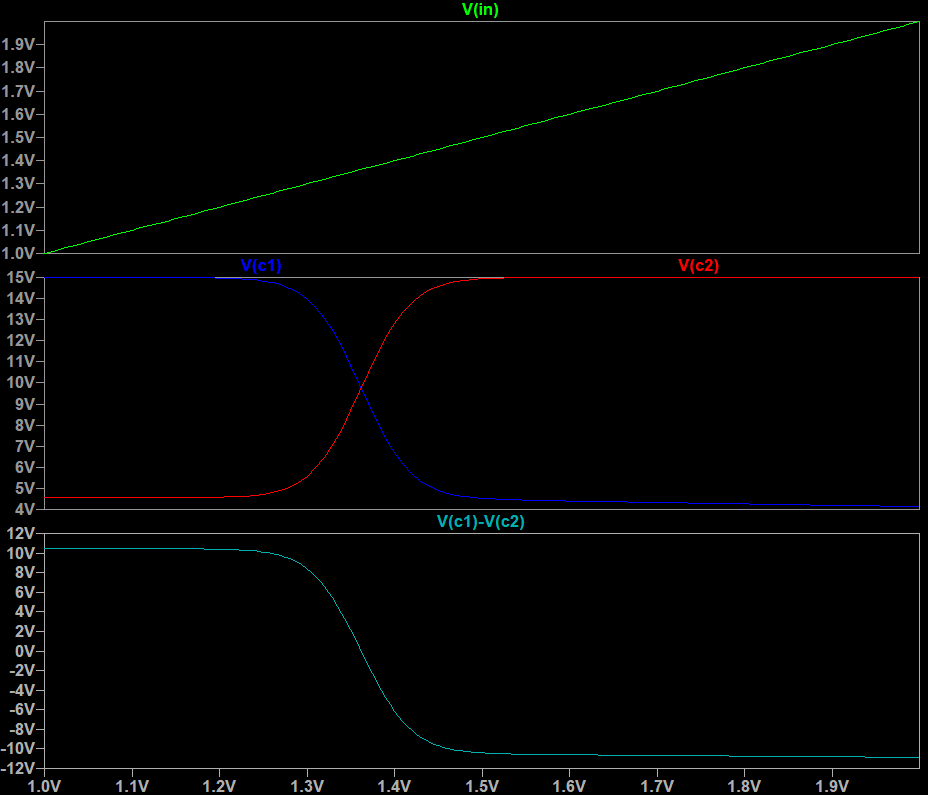
\includegraphics[width=10.0cm]{figures/exercise1plot2.png}
\caption{Είσοδος και Έξοδος Ενισχυτή με DC Sweep}\label{fig:ex1plot2}
\end{figure}

\subsection{Θεωρητική Ανάλυση}

\paragraph*{}

Όσων αφορά την θεωρητική ανάλυση, υιοθετούμε τις κλασικές παραδοχές \(\beta = 100\) και \(V_{BE} = 0.5 \ V\) για τα τρανζίστορ. Τότε βλέπουμε ότι για \(V_{in} = 0\) είναι \(V_{B1} = 0\) άρα το \(Q_1\) είναι σε αποκοπή και ισχύει \(V_{C1} = 15\ V\). Η \(V_{B2}\) υπολογίζεται από τον διαιρέτη τάσης:
\[
V_{B2} = V_2\frac{1k\ \Omega}{10k \ \Omega + 1 \ k\Omega} = 1.363\ V
\]
Συνεπώς, για το ρεύμα \(I_{C2}\) έχουμε:

\begin{gather*}
    I_{C2} = \beta I_{B2} = \beta \frac{V_{B2} - V_{BE} - V_1}{(\beta+1)R_5} = 1.047 \ mA
\end{gather*}
Άρα έχουμε:

\[
I_{E2} = \frac{\beta+1}{\beta}I_{C2} = 1.057 \ mA, \quad\quad V_{C2} = V_2 - I_{E2}R_7 = 4.53\ V
\]
Συνεπώς η τάση στην έξοδο είναι:
\[
V_{out} = V_{C1} - V_{C2} = 10.47 \ V
\]
Έχουμε επίσης:
\[
V_A = V_1 + I_{E2}R_5 = 0.855\ V
\]
άρα η ελάχιστη τάση εισόδου \(V_{in}\) για την οποία το \(Q_1\) βγαίνει από την αποκοπή είναι:
\[
V_{in,\min} = V_A + V_{BE} = 1.355 \ V
\]

Όταν \(V_{in} - V_{B2} = 1.363 \ V\) θα έχουμε ίσα ρεύματα στους συλλέκτες:
\[
I_{C1} = I_{C2} = \beta I_{B} = 0.523 \ mA
\]
Τότε έχουμε:
\[
V_{C1} = V_{C2} = V_2 - I_{C1,C2}R_{6,7} = 9.77 \ V, \quad\quad V_{out} = V_{C1} - V_{C2} = 0
\]

Για την μεταβολή της τάσης στον συλλέκτη του \(Q_1\) έχουμε:
\[
V_{C1} = \frac{\beta R_{C1}}{2(r_{bb'}+r_{b'e})}(V_{in2}-V_{in1}) = -52.05\Delta V_{in} \Rightarrow \Delta V_{in} = \frac{5.23}{52.05} = 1.005 \ V 
\]
Συνεπώς, όταν η \(V_{in}\) αυξάνεται κατά \(0.1004 \ V\), η τάση στην συλλέκτη του \(Q_2\) ανεβαίνει κατά \(5.23 \ V\) ενώ στον συλλέκτη του \(Q_1\) κατεβαίνει κατά \(5.23 \ V\).

Για \(V_{in} = V_{in,\max} = 2.7 \ V\) έχουμε:
\[
I_{C1} = \frac{\beta (V_{in,\max} - V_{BE} - V_1)}{(\beta + 1)R_5} = 1.134 \ mA
\]
άρα τότε:
\[
V_{C1} = V_2 - I_{C1}R_6 = 3.66\ V
\]

Συνοψίζοντας, τα θεωρητικά αποτελέσματα για την σχέση των τιμών εισόδου και εξόδου φαίνονται στον πίνακα:
\begin{center}
\begin{tabular}{|c|c|c|c|}
\hline
\(V_{in}\) & \(V_{C1}\) & \(V_{C2}\) & \(V_{out}\)  \\
\hline
\(0\ V - 1.355 \ V\) & \(15 \ V\) & \(4.54 \ V\) & \(10.46 \ V\)  \\
\hline
\(1.363 \ v\) & \(9.77 \ V\) & \(9.57 \ V\) & \(0 \ V\)  \\
\hline
\(1.463 \ V\) & \(4.54 \ V\) & \(15 \ V\) & \(-10.46 \ V\) \\
\hline
\(2.7 \ V\) & \(3.66 \ V\) & \(15 \ V\) & \(-11.34 \ V\) \\
\hline
\end{tabular}
\end{center}

Τα παραπάνω αποτελέσματα είναι πολύ κοντινά και με τα αποτελέσματα των προσομοιώσεων και με τις τιμές που μετρήθηκαν στο εργαστήριο.



\section{Βήμα 8}

\paragraph*{} Υλοποιήθηκε το κύκλωμα 1-8 του φυλλαδίου, χωρίς την πηγή τάσης, όπως φαίνεται στο σχήμα \ref{fig:ex1circuit3}.

\begin{figure}[h]
\centerfloat%
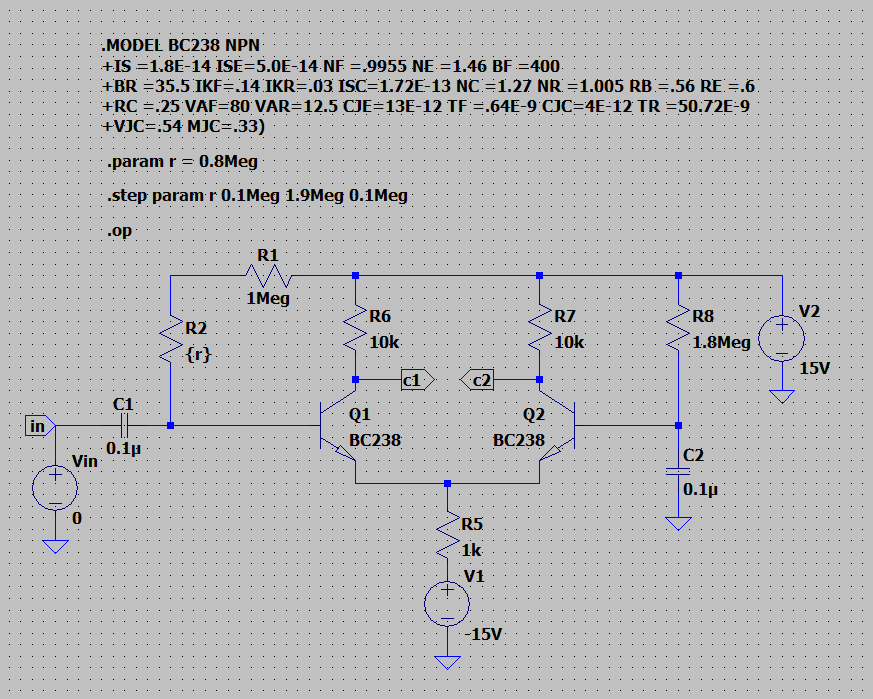
\includegraphics[width=12.0cm]{figures/exercise1circuit3.png}
\caption{Κύκλωμα 1-8}\label{fig:ex1circuit3}
\end{figure}

Με παραμετρική ανάλυση στην παράμετρο \(r\) της αντίστασης \(R_2\) βρέθηκε ότι η τάση στους συλλέκτες των τρανζίστορ γίνονται ίσες για \(r = 0.8 \ M\Omega\), όπως φαίνεται στο σχήμα \ref{fig:ex1plot3}.

\begin{figure}[h]
\centerfloat%
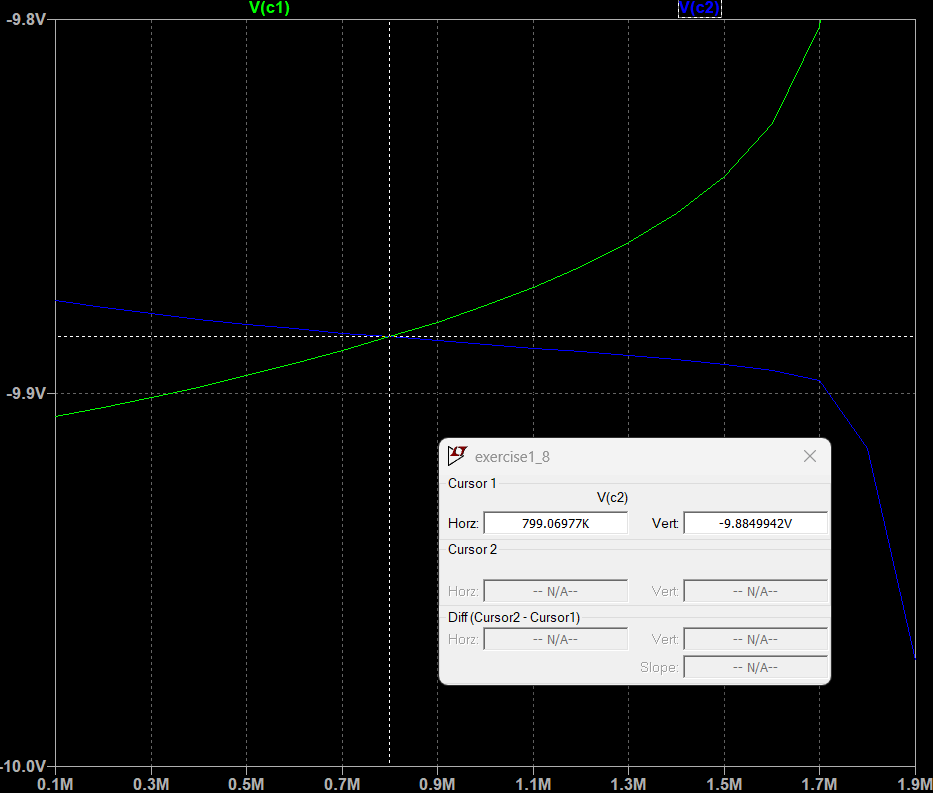
\includegraphics[width=12.0cm]{figures/exercise1plot3.png}
\caption{Ισοστάθμιση Τάσεων Συλλεκτών}\label{fig:ex1plot3}
\end{figure}

Με αυτήν την τιμή της παραμέτρου \(r\) και με AC πηγή τάσης εισόδου πλάτους \(0.1 \ V\) peak to peak, οι τάσεις εισόδου και εξόδου φαίνονται στο σχήμα \ref{fig:ex1plot4}.

\begin{figure}[h]
\centerfloat%
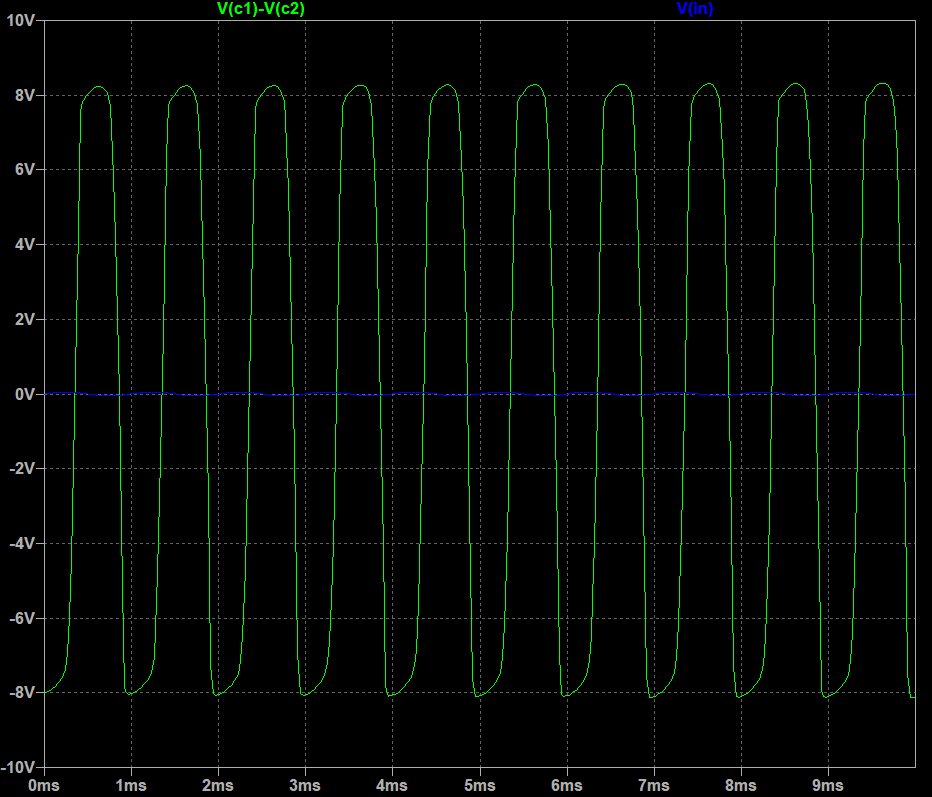
\includegraphics[width=12.0cm]{figures/exercise1plot4.png}
\caption{Τάσεις Εισόδου και Εξόδου}\label{fig:ex1plot4}
\end{figure}

Με AC ανάλυση για την πηγή \(V_{in}\) στο εύρος συχνοτήτων \(100 \ Hz - 1\ MHz\) η ενίσχυση του σήματος εισόδου φαίνεται στο σχήμα \ref{fig:ex1plot5}.

\begin{figure}[h]
\centerfloat%
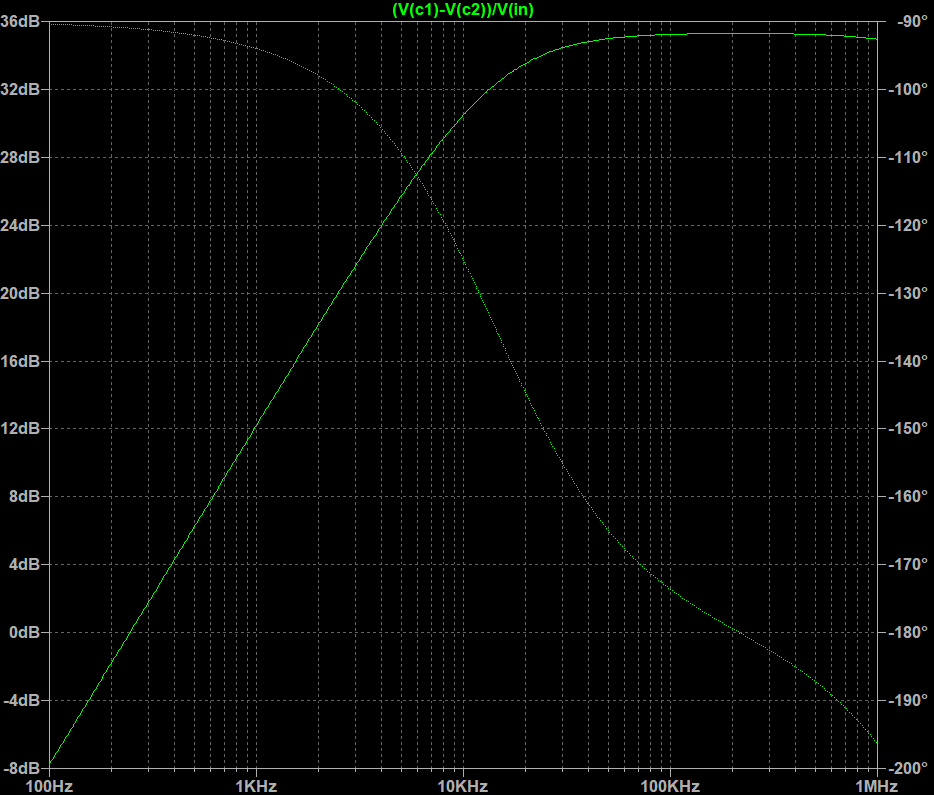
\includegraphics[width=12.0cm]{figures/exercise1plot5.png}
\caption{Ενίσχυση στις Συχνότητες \(100 \ Hz - 1 \ M Hz\)}\label{fig:ex1plot5}
\end{figure}

%%%%%%%%%%%%%%%%%%%%%%%% Exercise 3 %%%%%%%%%%%%%%%%%%%%%%%%
%%%%%%%%%%%%%%%%%%%%%%%%%%%%%%%%%%%%%%%%%%%%%%%%%%%%%%%%%%%%

\chapter{Εργαστηριακή Άσκηση 3}

\section{Βήμα 10}

\paragraph*{} Υλοποιήθηκε το κύκλωμα 3-3 του φυλλαδίου όπως φαίνεται στην εικόνα \ref{fig:ex3circuit1}.

\begin{figure}[H]
\centerfloat%
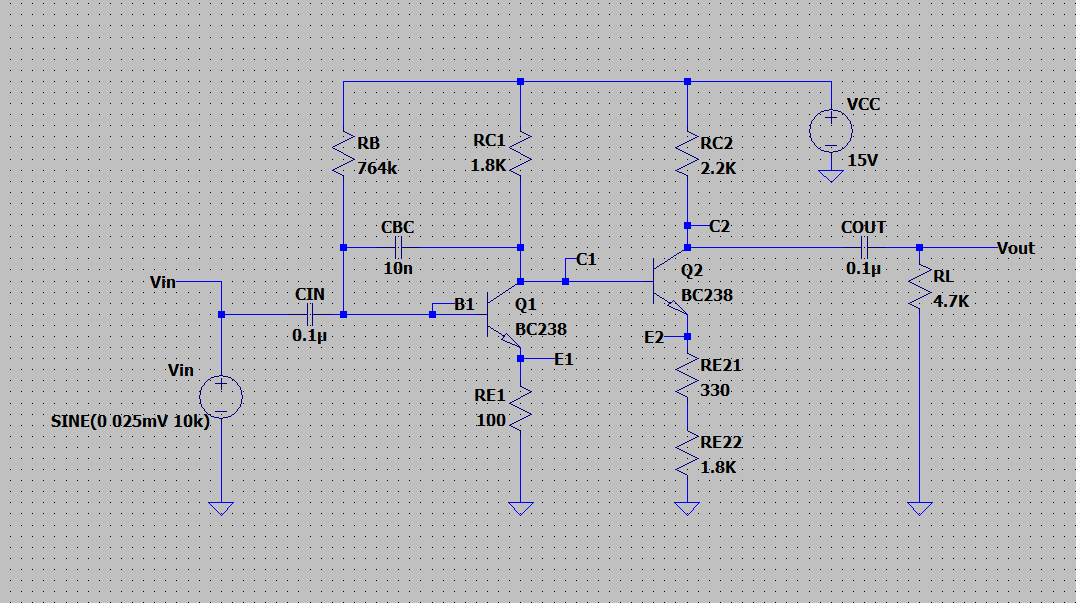
\includegraphics[width=15.0cm]{figures/exercise3circuit1.png}
\caption{Κύκλωμα 3-3}\label{fig:ex3circuit1}
\end{figure}

 Η τιμή της αντίστασης \(R_B\) επιλέχθηκε με παραμετρική ανάλυση, ώστε η τάση στον συλλέκτη του \(Q_1\) να είναι ίση με \(5 \ V\), όπως φαίνεται στο διάγραμμα του σχήματος \ref{fig:ex3plot1}.

\begin{figure}[H]
\centerfloat%
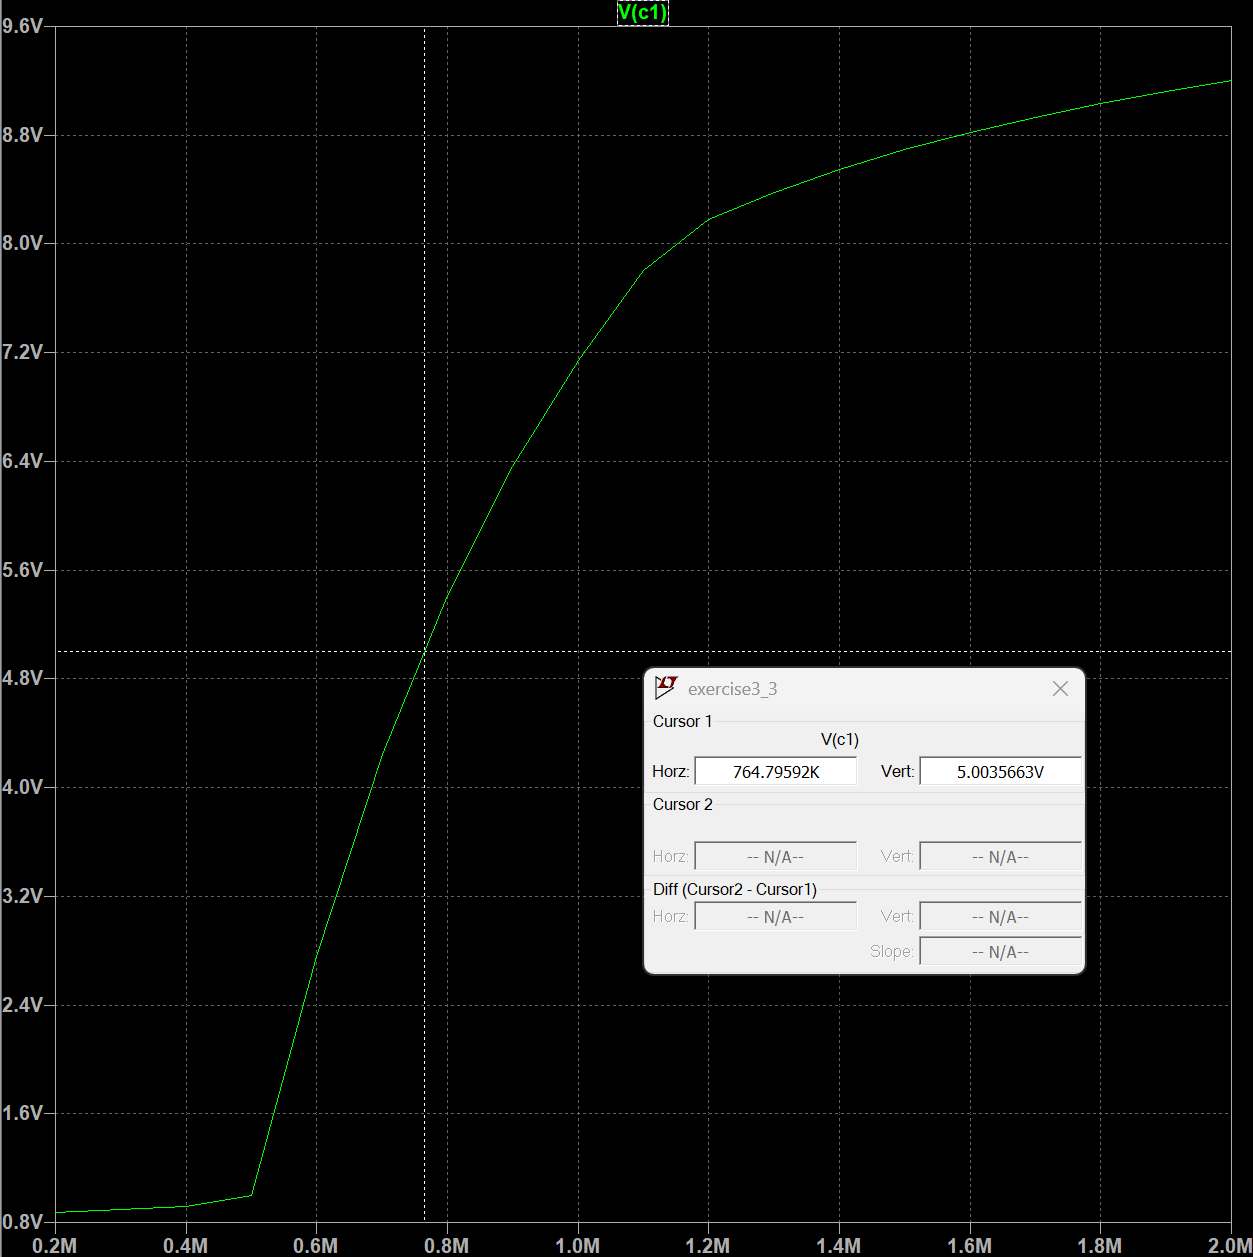
\includegraphics[width=12.0cm]{figures/exercise3plot1.png}
\caption{Ρύθμιση της αντίστασης \(R_B\)}\label{fig:ex3plot1}
\end{figure}

Οι τάσεις στους ακροδέκτες των δύο τρανζίστορ φαίνονται στο σχήμα \ref{fig:ex3plot2}.

\begin{figure}[H]
\centerfloat%
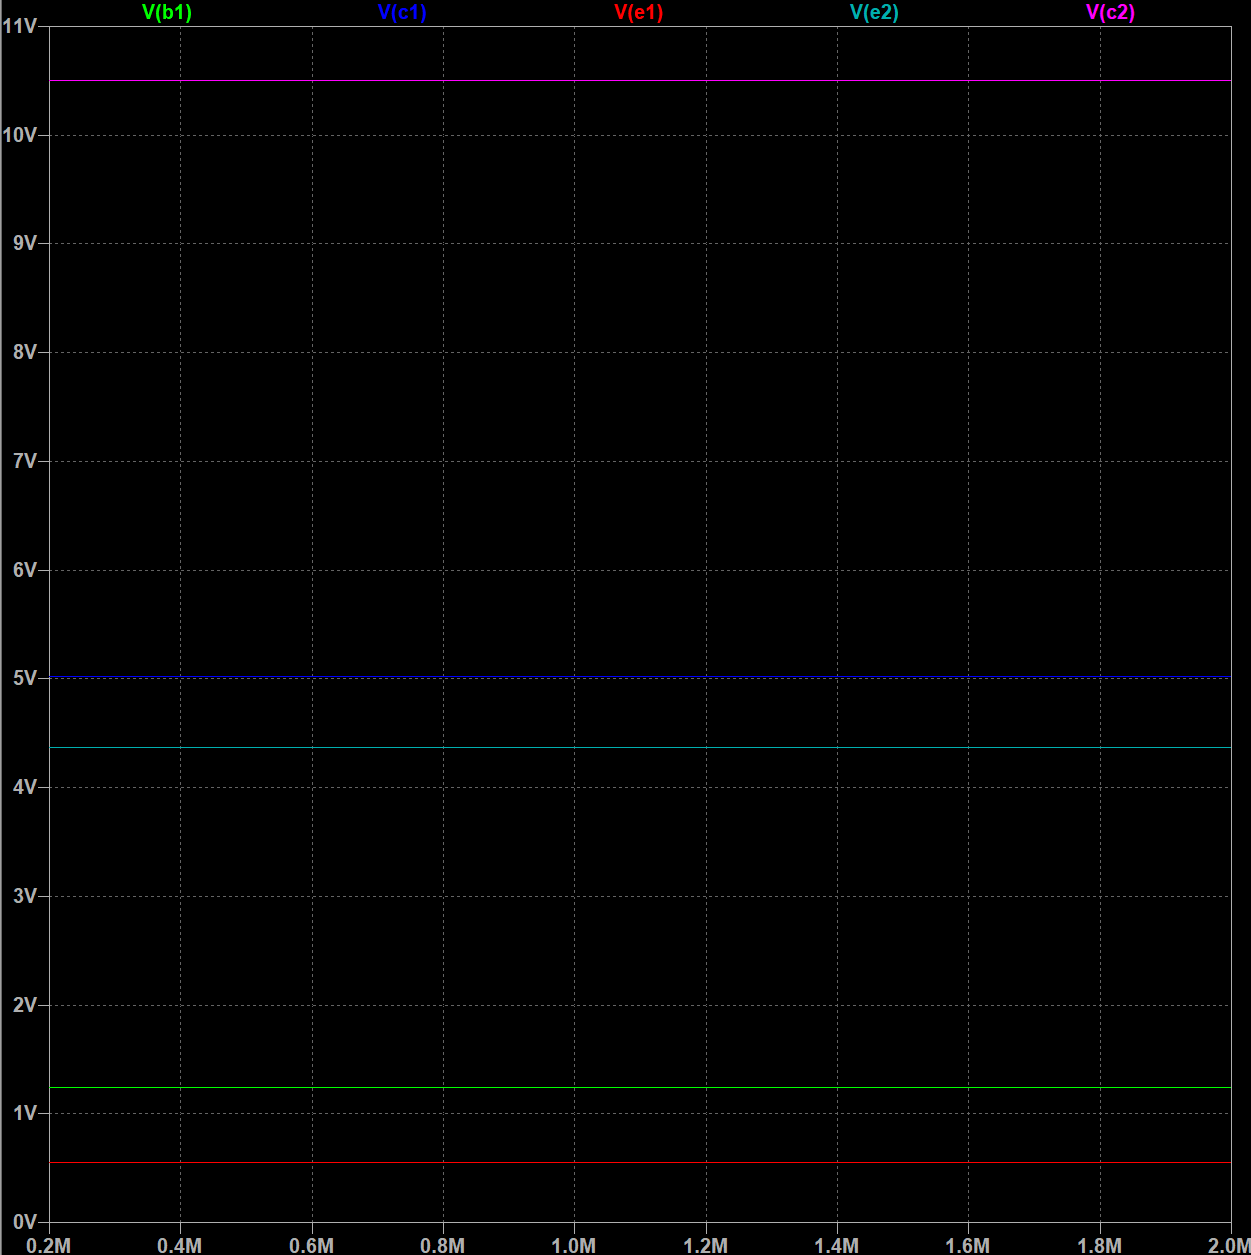
\includegraphics[width=12.0cm]{figures/exercise3_1plot_DC.png}
\caption{Τάσεις στους ακροδέκτες των τρανζίστορ}\label{fig:ex3plot2}
\end{figure}

Βάλαμε σήμα \(50 \ mV\) peak to peak και συχνότητας \(10 \ kHz\) στην είσοδο του κυκλώματος. Η είσοδος και η έξοδος φαίνονται στο διάγραμμα του σχήματος \ref{fig:ex3plot3}. Η ενίσχυση που παρατηρείται είναι ίση με \(3.92\).

\begin{figure}[H]
\centerfloat%
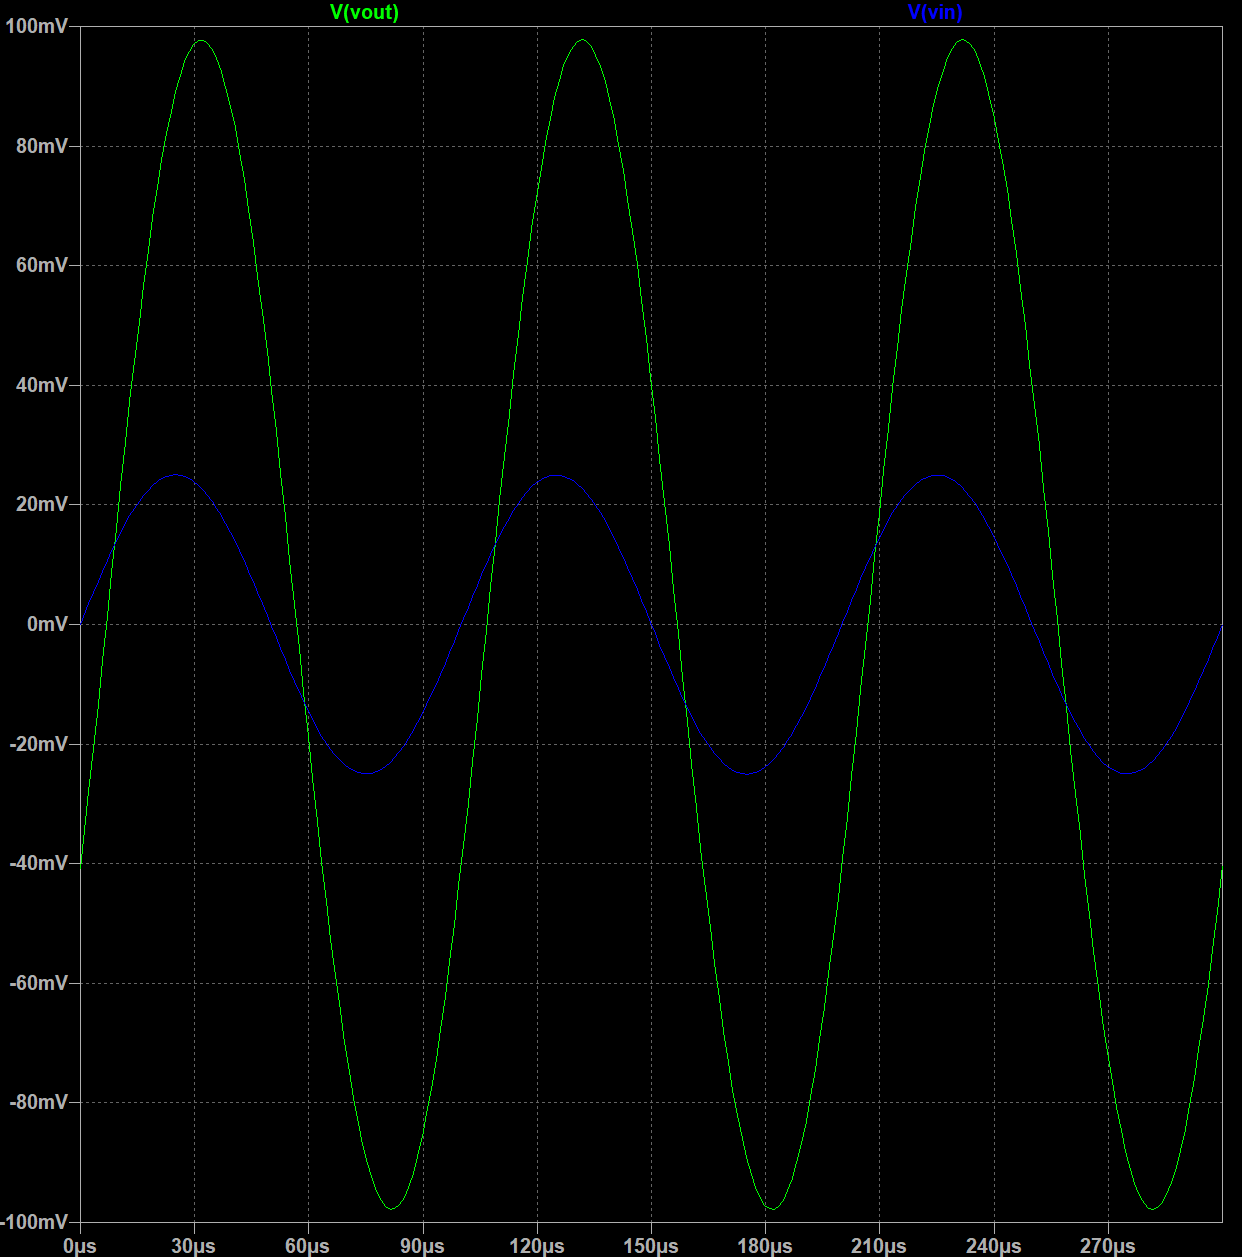
\includegraphics[width=12.0cm]{figures/exercise3_1transient.png}
\caption{Είσοδος και Έξοδος (χωρίς πυκνωτή \(C_{E2}\))}\label{fig:ex3plot3}
\end{figure}

Μεταβλήθηκε το πλάτος του σήματος εισόδου μέχρι η έξοδος να αρχίσει να παραμορφώνεται, όπως φαίνεται στο σχήμα \ref{fig:ex3plot4}. Το μέγιστο πλάτος εισόδου για το οποίο δεν υπάρχει παραμόρφωση στην έξοδο είναι \(600 \ mV\) (ή \(1.2 \ V\) peak to peak).

\begin{figure}[H]
\centerfloat%
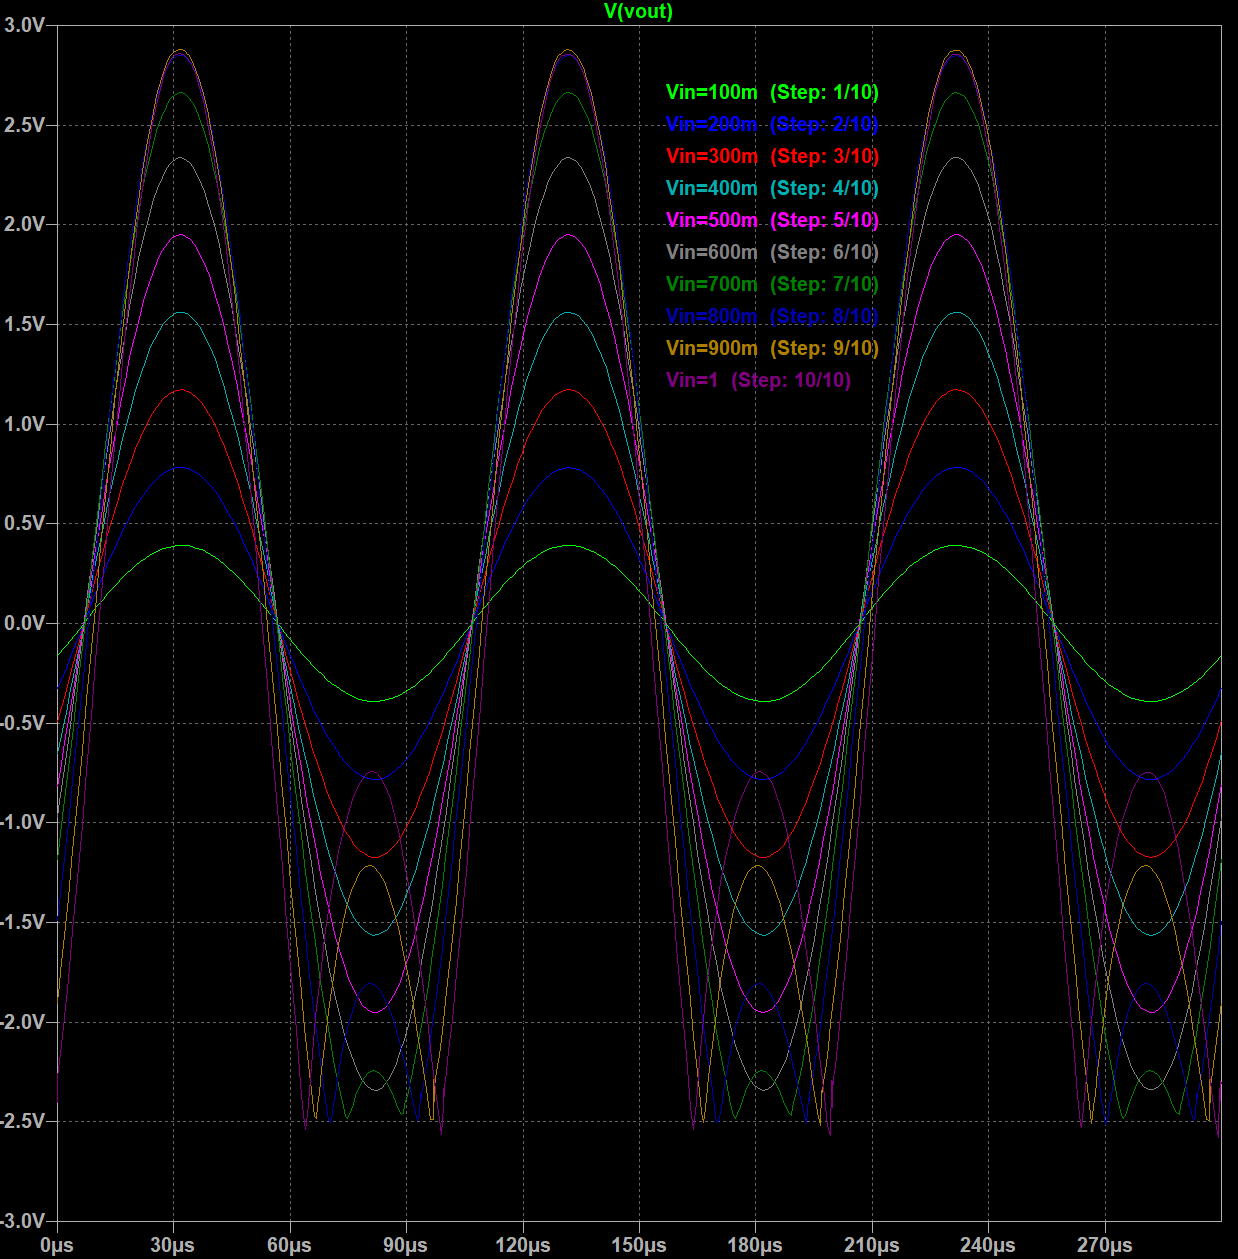
\includegraphics[width=12.0cm]{figures/exercise3_1apokopi.png}
\caption{Μεταβολή του πλάτους εισόδου (χωρίς πυκνωτή \(C_{E2}\))}\label{fig:ex3plot4}
\end{figure}

Συνδέθηκε ο πυκνωτής \(C_{E2}\), όπως φαίνεται στο σχήμα \ref{fig:ex3circuit2}.
\begin{figure}[H]
\centerfloat%
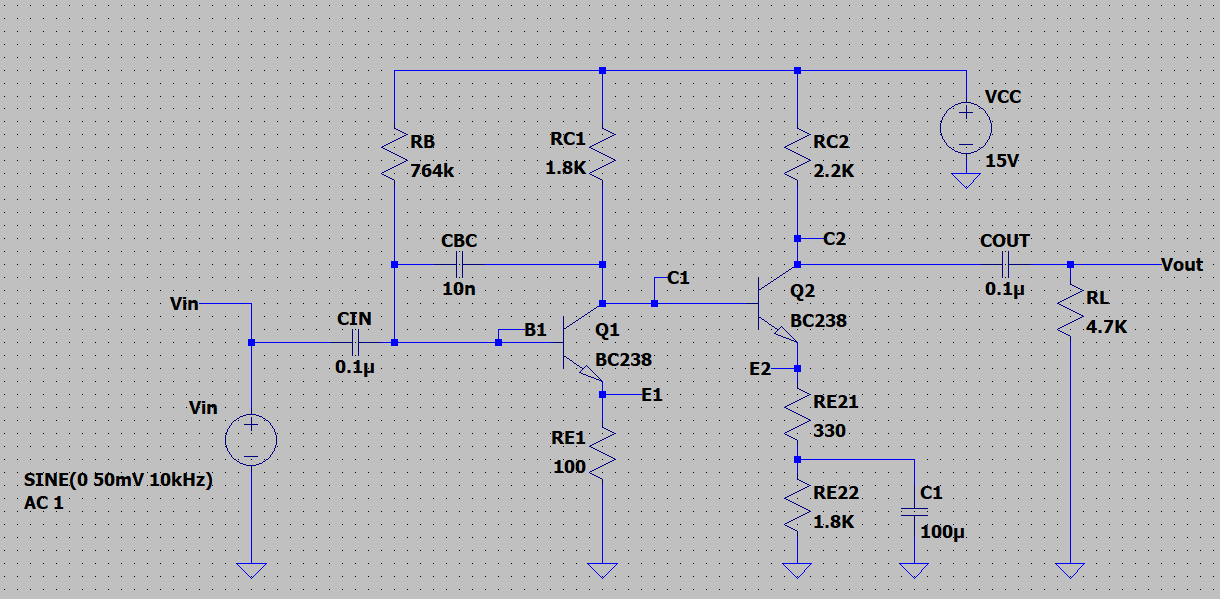
\includegraphics[width=12.0cm]{figures/exercise3circuit2.png}
\caption{Κύκλωμα 3-3 με πυκνωτή \(C_{E2}\)}\label{fig:ex3circuit2}
\end{figure}

Μεταβλήθηκε και πάλι το πλάτος εισόδου μέχρι να παρατηρηθεί παραμόρφωση στην έξοδο, η οποία ξεκίνησε για πλάτος εισόδου ίσο με \(150 \ mV\) (ή \(300\ mV\) peak to peak), όπως φαίνεται στο σχήμα \ref{fig:ex3plot5}.
\begin{figure}[H]
\centerfloat%
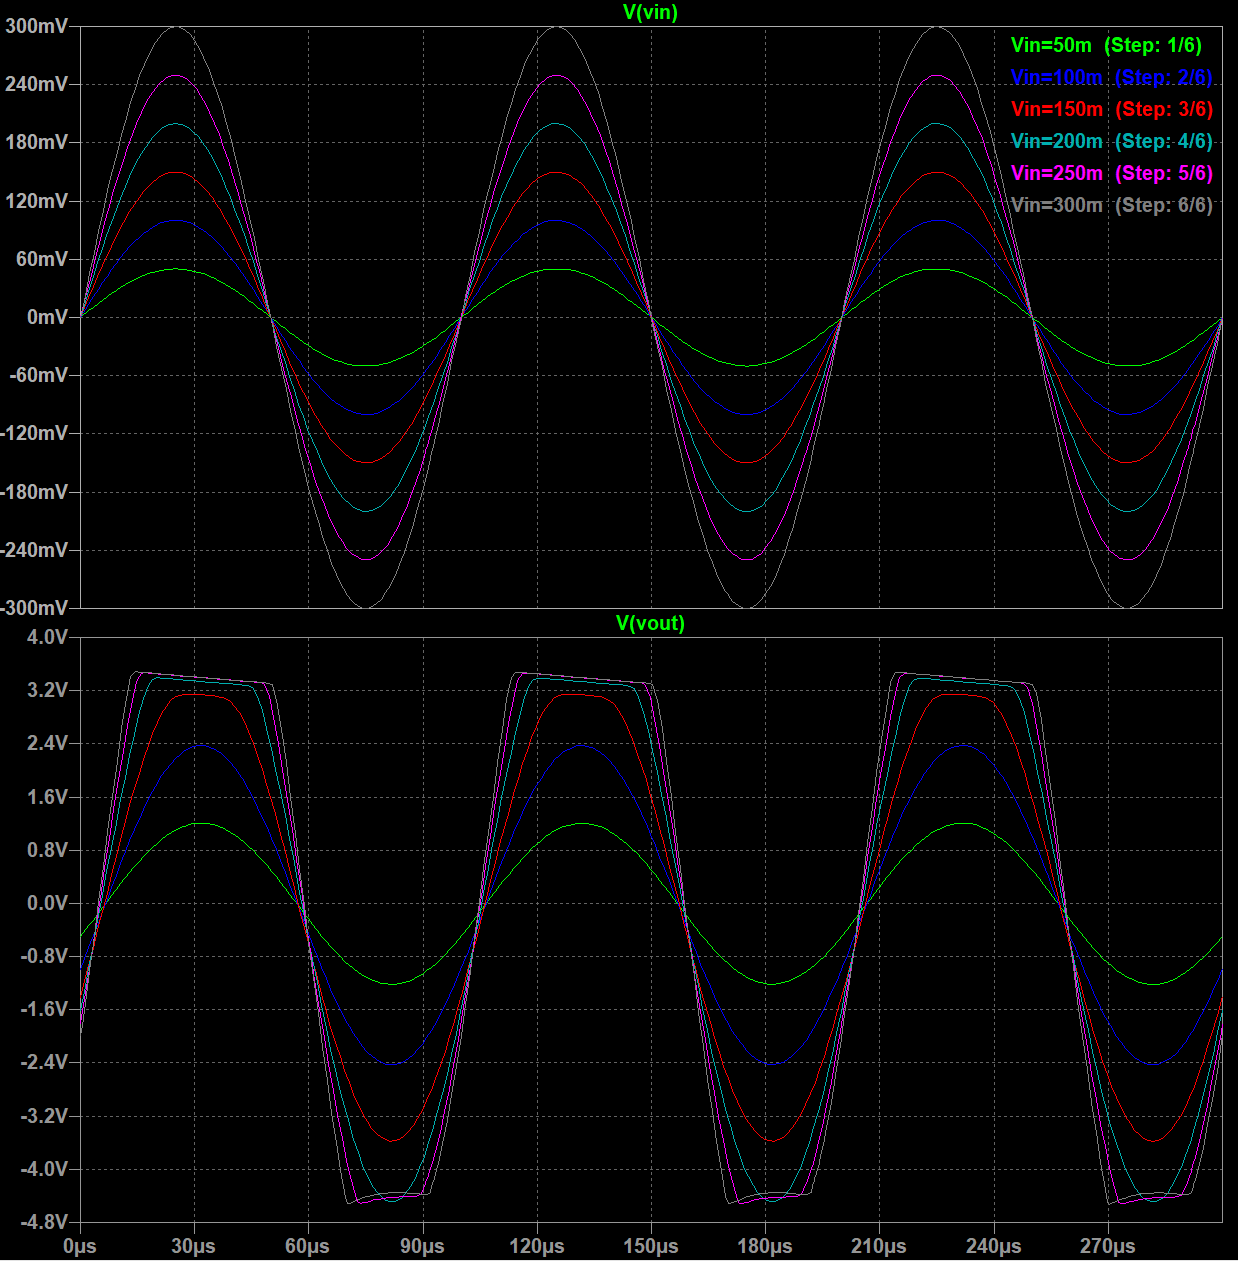
\includegraphics[width=12.0cm]{figures/exercise3_2apokopi.png}
\caption{Μεταβολή του πλάτους εισόδου (με πυκνωτή \(C_{E2}\))}\label{fig:ex3plot5}
\end{figure}

Προσθέτοντας τον κλάδο ανάδρασης $R_F$-$C_F$ έχουμε το σχήμα \ref{fig:ex3circuit3}.
\begin{figure}[H]
\centerfloat
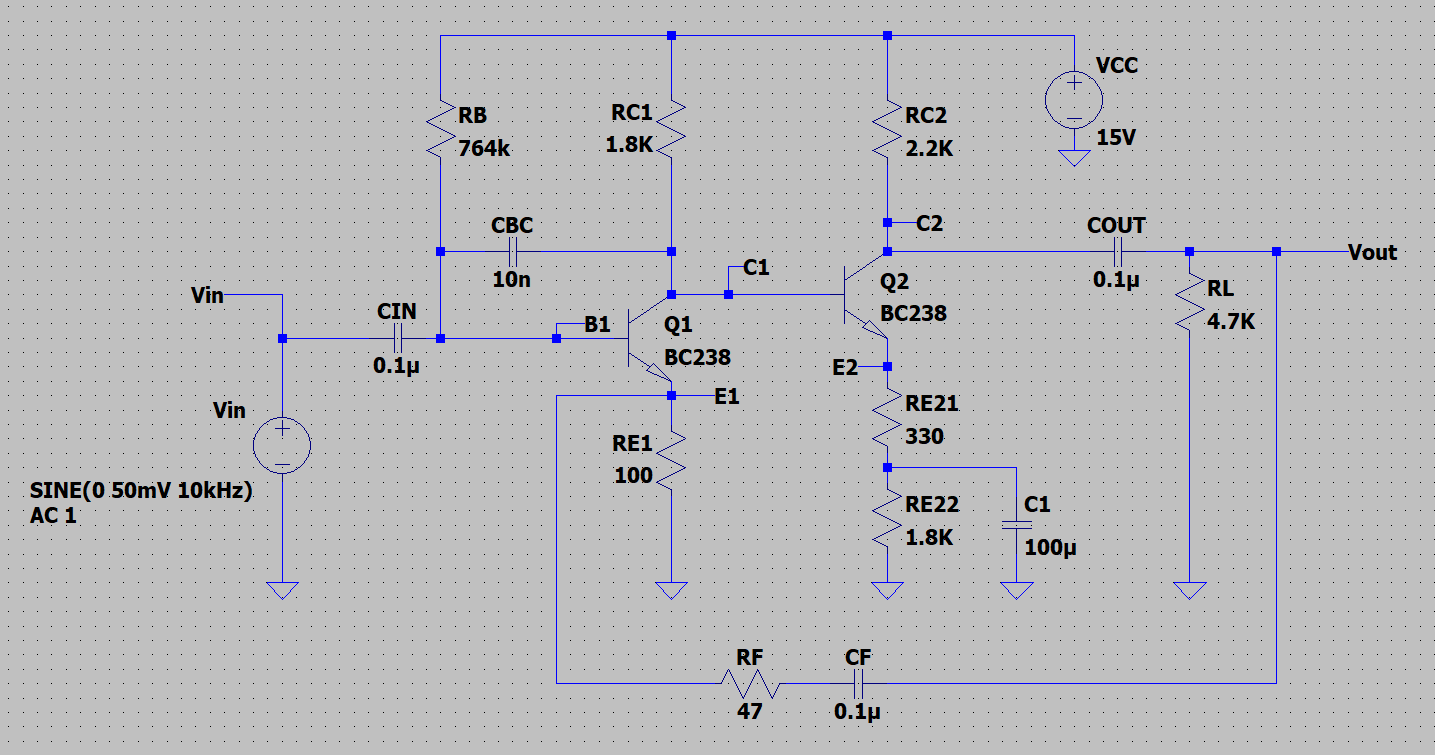
\includegraphics[width=12.0cm]{figures/exercise3circuit3.png}
\caption{Κύκλωμα 3-3 με ανάδραση}
\label{fig:ex3circuit3}
\end{figure}

Παρατηρούμε την εξής γραφική παράσταση \ref{fig:ex3plot6}.
\begin{figure}[H]
\centerfloat
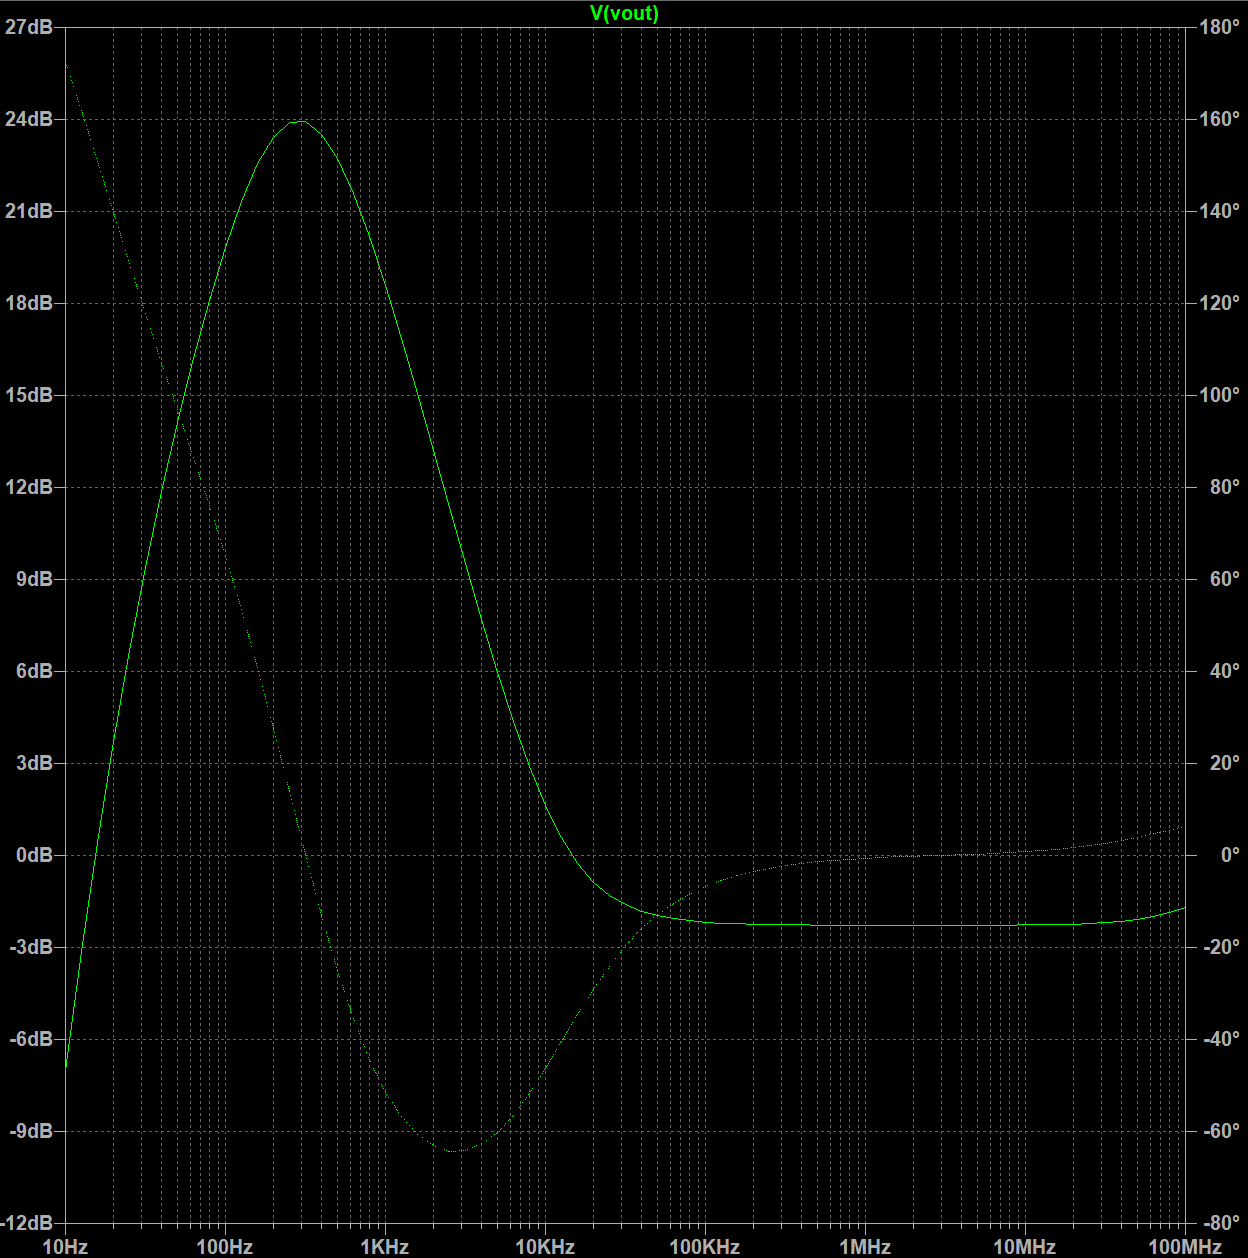
\includegraphics[width=12.0cm]{figures/exercise3_3plot_feedback.png}
\caption{AC sweep για την έξοδο του κυκλώματος 3-3 με ανάδραση}
\label{fig:ex3plot6}
\end{figure}

Ακολουθεί το κύκλωμα 3-4 του φυλλαδίου του εργαστηρίου όπου οι καινούριες τιμές τάσης των δύο τρανζίστορ είναι ως εξής:
\begin{figure}[H]
\centerfloat
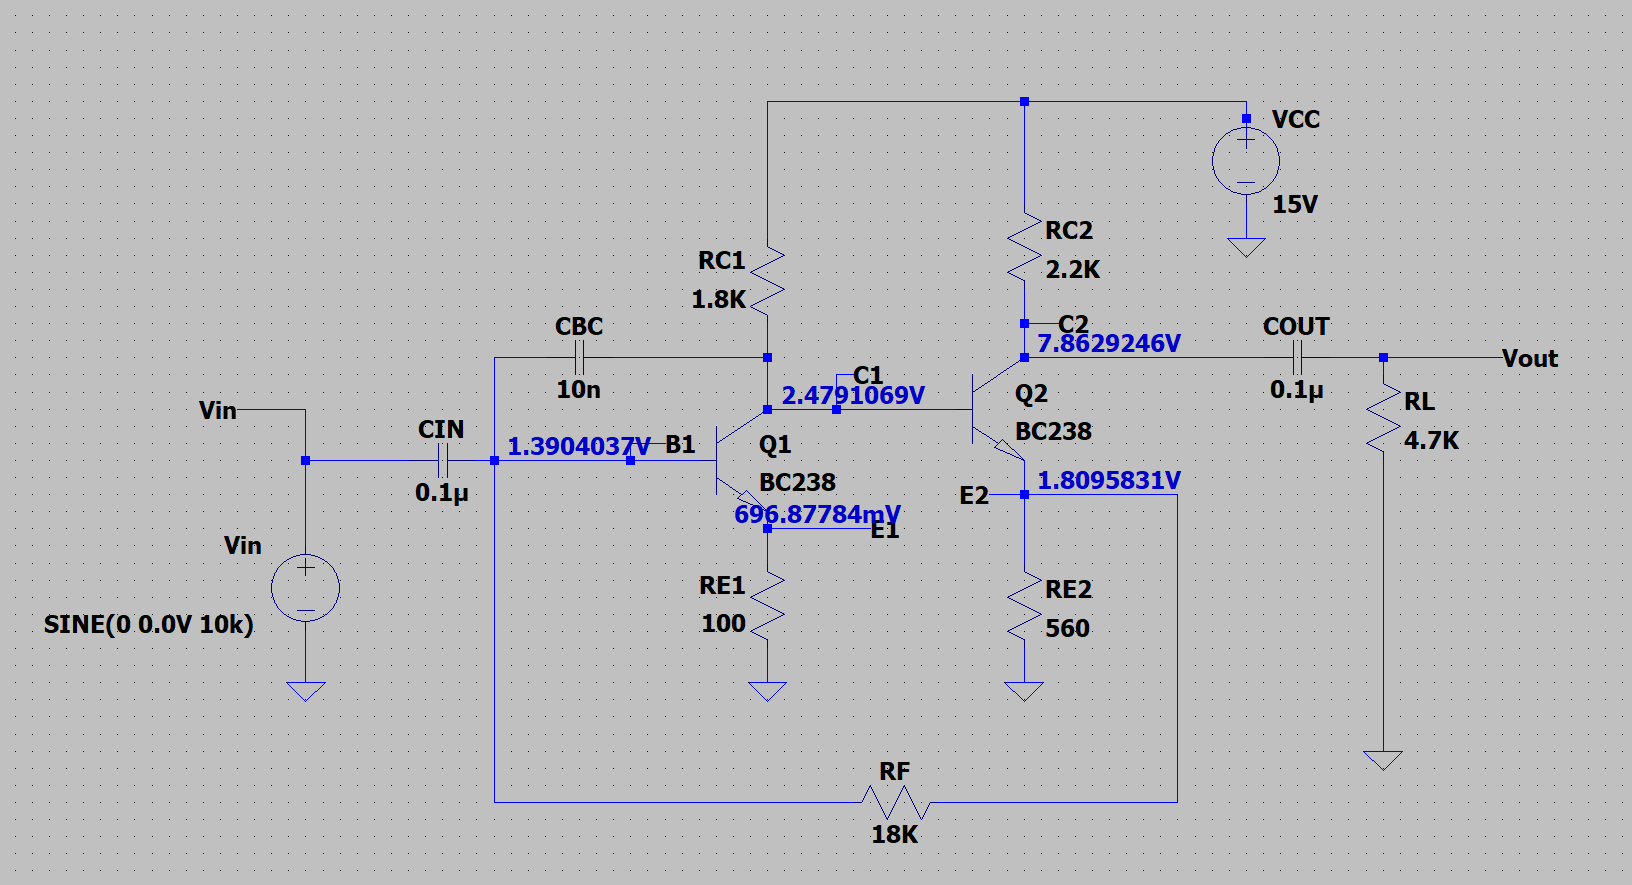
\includegraphics[width=12.0cm]{figures/exercise3circuit4.png}
\caption{Κύκλωμα 3-4}
\label{fig:ex3circuit4}
\end{figure}
Μετά από AC ανάλυση προκύπτει η παρακάτω γραφική παράσταση:
\begin{figure}[H]
\centerfloat
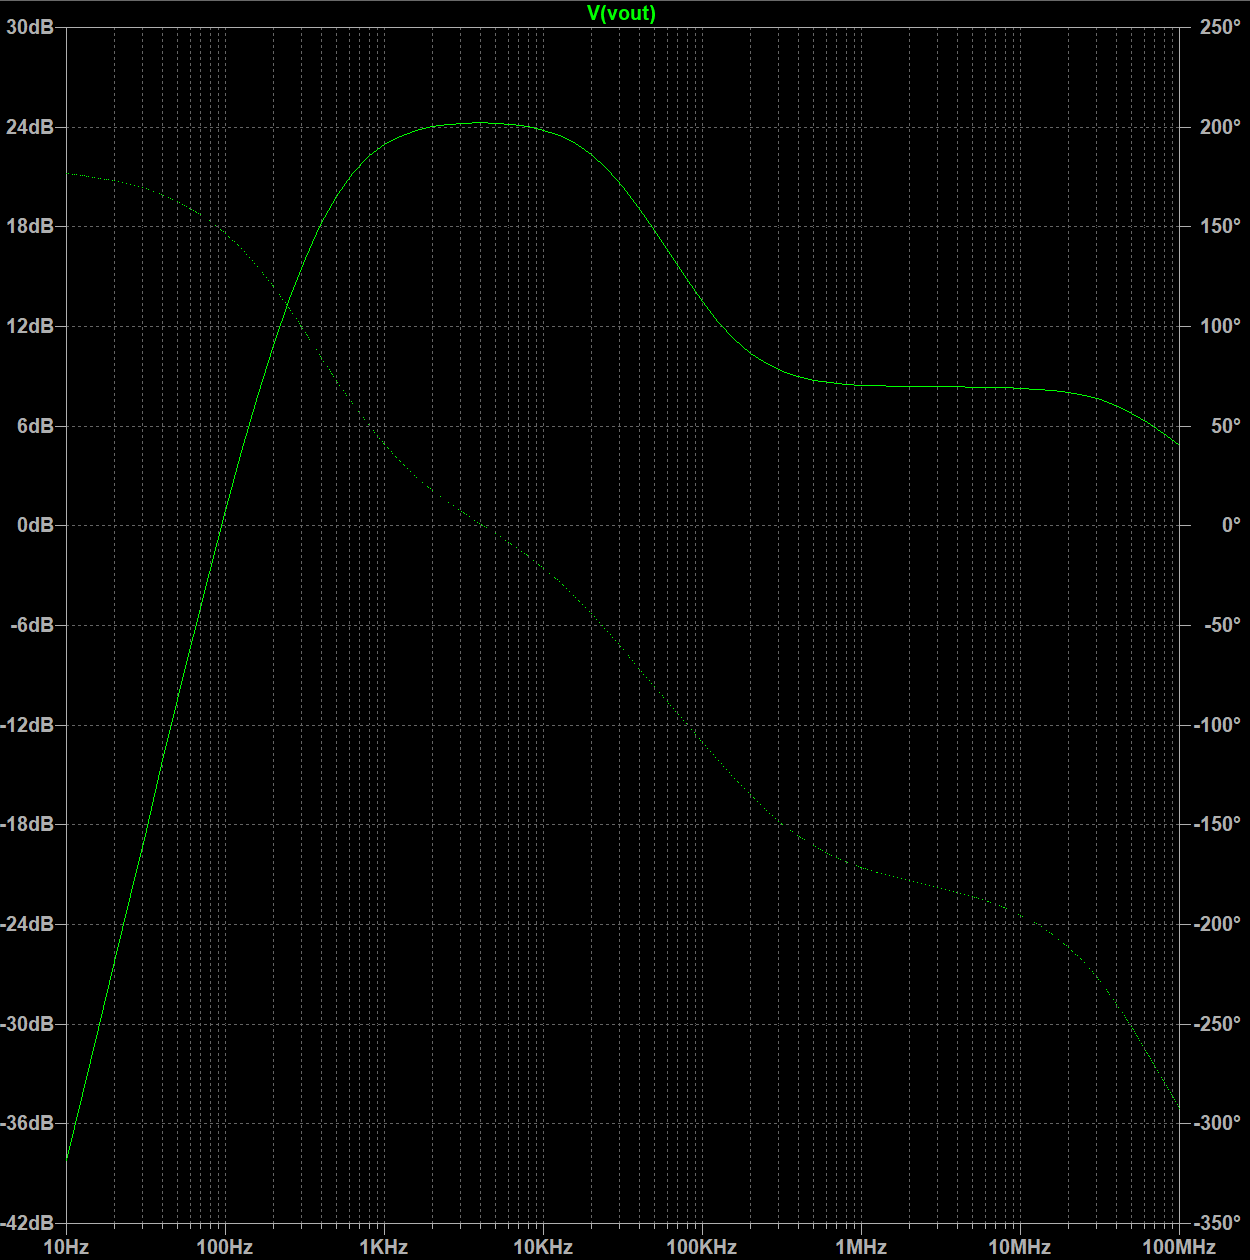
\includegraphics[width=12.0cm]{figures/exercise3_4plot.png}
\caption{AC sweep στην έξοδο του κυκλώματος 3-4}
\label{fig:ex3plot4}
\end{figure}
Η χρονική ανάλυση του κυκλώματος έχει ως εξής: 
\begin{figure}[H]
\centerfloat
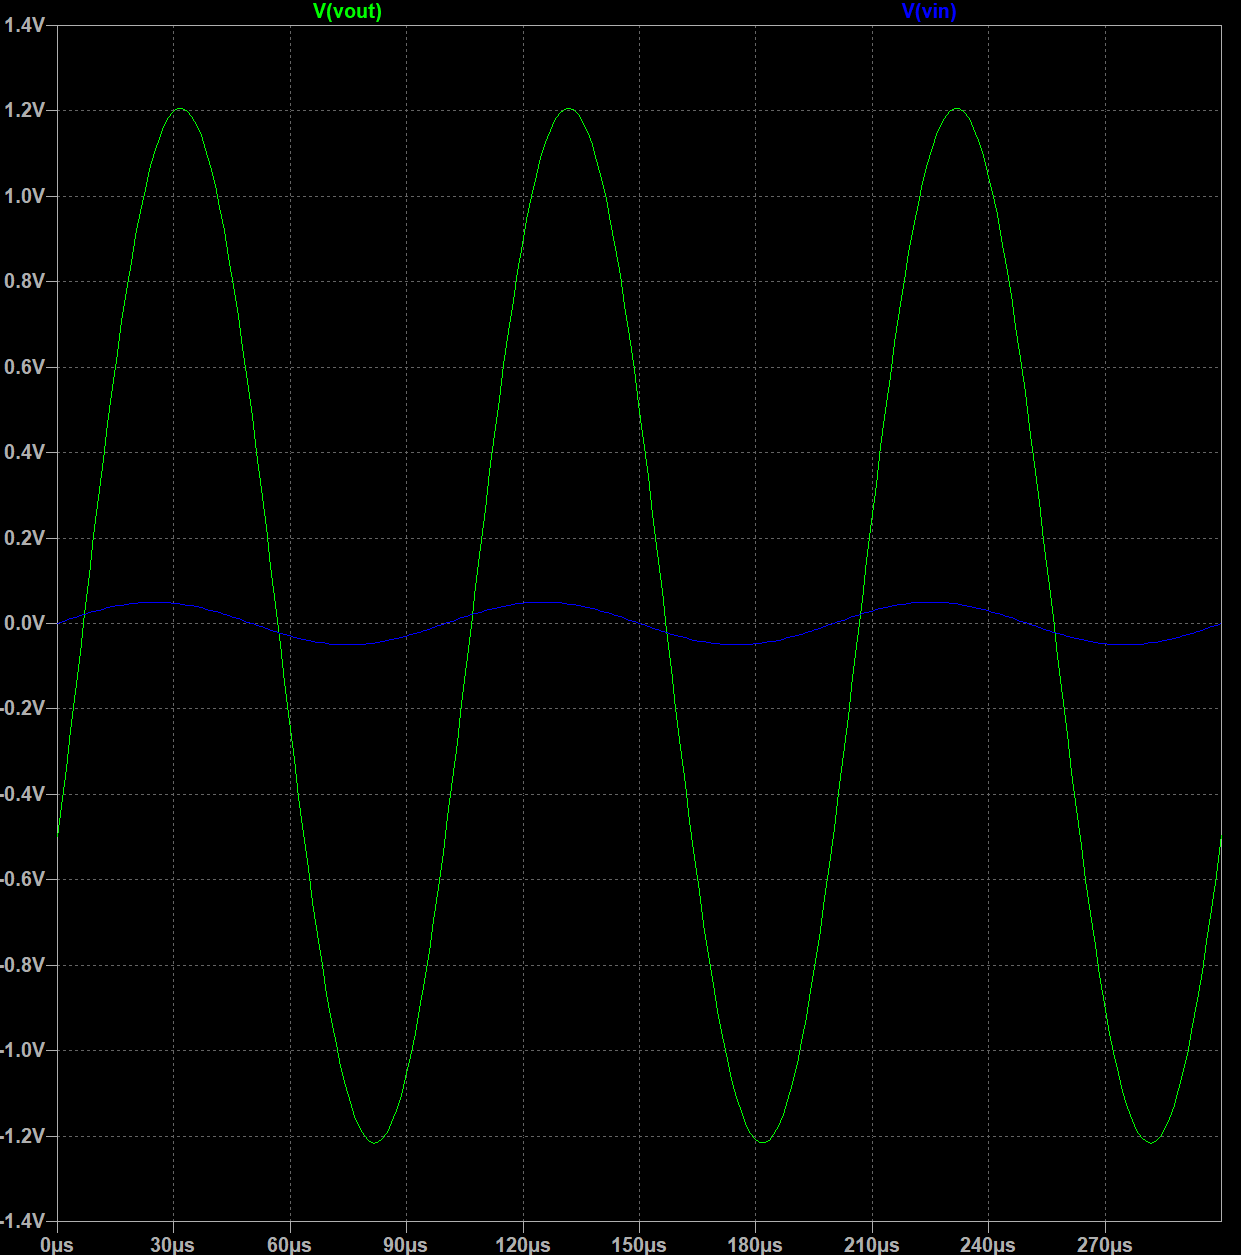
\includegraphics[width=12.0cm]{figures/exercise3_4transient.png}
\caption{Χρονική ανάλυση του κυκλώματος 3-4}
\label{fig:ex3plottransient}
\end{figure}

\section{Βήμα 11}

\paragraph*{}

Για την θεωρητική ανάλυση των κυκλωμάτων θεωρούμε τις τιμές:

\[
V_{BE} = 0.672\ V, \quad \beta = 333
\]
οι οποίες μετρήθηκαν στο εργαστήριο. Ισχύουν οι σχέσεις:

\begin{gather*}
I_{C1} = \frac{V_{CC} - V_{C1}}{R_{C1}} =  5.55\ mA \\
I_{E1} = \frac{\beta + 1}{\beta} I_C = 5.56\, mA \\
V_{E1} = R_{E1}I_{E1} = 0.556 \ V \\
V_{B1} = V_{E1} + V_{BE} = 1.228 \ V \\
I_{B1} = \frac{I_{C1}}{\beta} = 0.017 \ mA
\end{gather*}
άρα για την \(R_B\) έχουμε:
\[
R_B = \frac{V_{CC}-V_{B1}}{I_{B1}} = 810.11\ kA
\]

Στο τρανζίστορ \(Q_1\) ισχύει:

\begin{gather*}
    V_{C1} = 5\ V \\
    V_{B1} = 1.228 \ V \\
    V_{E1} = 0.556 \ V \\
    I_{C1} = 5.55 \ mA \\
    I_{B1} = 0.017 \ mA
\end{gather*}

Στο τρανζίστορ \(Q_2\) ισχύει:

\begin{gather*}
    V_{B2} = V_{C1} = 5\ V \\
    V_{E2} = V_{B2} - V_{BE} = 4.32 \ V \\
    I_{E2} = \frac{V_{E2}}{R_{E21} + R_{E22}} = 2.028 \ mA \\
    I_{C2} = \frac{\beta}{\beta + 1}I_{E2} = 2.022 \ mA \\
    I_{B2} = \frac{I_{C2}}{\beta} = 0.006 \ mA
\end{gather*}

Για τον ενισχυτή έχουμε:

\begin{gather*}
    g_{m1} = \frac{I_{C1}}{V_T} = 0.213 \ A/V \\
    g_{m2} = \frac{I_{C2}}{V_T} = 0.077 \ A/V \\
    r_{b'e1} = \frac{\beta}{g_{m1}} = 1563 \ \Omega \\
    r_{b'e2} = \frac{\beta}{g_{m2}} = 4324 \ \Omega
\end{gather*}

Συνεπώς για τις δύο βαθμίδες ενίσχυσης ισχύει:

\begin{gather*}
    A_1 = - \frac{R_{C1}'}{R_{E1}'} = - \frac{1.8\ k\Omega \ \| \ (r_{b'e2}+(\beta + 1)(R_{E21}+R_{E22}))}{100 \ \Omega \ \| \ (47 \ \Omega + 2200 \ \Omega \| 4700 \ \Omega)} = -19.11 \\
    A_2 = - \frac{\beta R_{C2}'}{R_{E2}'} = -\frac{333 (220 \Omega\| 100\Omega+47\Omega\|4700\Omega)}{1800\Omega \| (r_{b'e2}+(\beta+1)2130\Omega)} = -21.33
\end{gather*}

Για την συνολική ενίσχυση με ανάδραση έχουμε:
\begin{gather*}
    F = \frac{R_{E1}}{R_{E1}+R_F} = 0.68 \\
    A_F = \frac{A_1A_2}{1+A_1A_2F} = 1.465
\end{gather*}

\section{Βήμα 12}

\paragraph*{} Στα σχήματα \ref{fig:ex3experiment1} και \ref{fig:ex3experiment2} φαίνονται οι μετρήσεις του εργαστηριακού πειράματος για την άσκηση 3.


\begin{figure}[h]
\centerfloat%
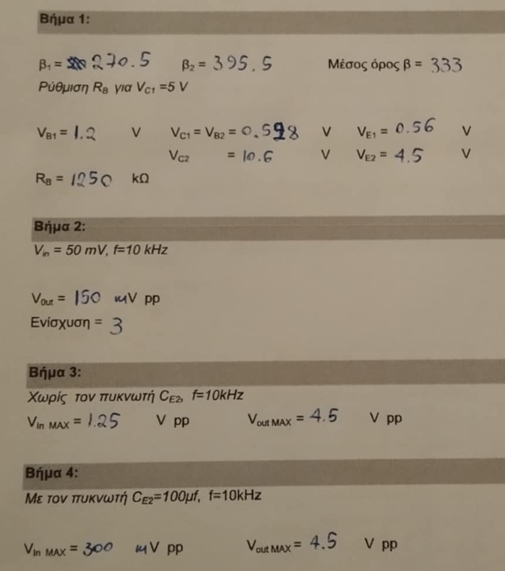
\includegraphics[width=15.0cm]{figures/exercise3experiment1.png}
\caption{Μετρήσεις Εργαστηριακής Άσκησης 3 (πρώτη σελίδα)}\label{fig:ex3experiment1}
\end{figure}


\begin{figure}[h]
\centerfloat%
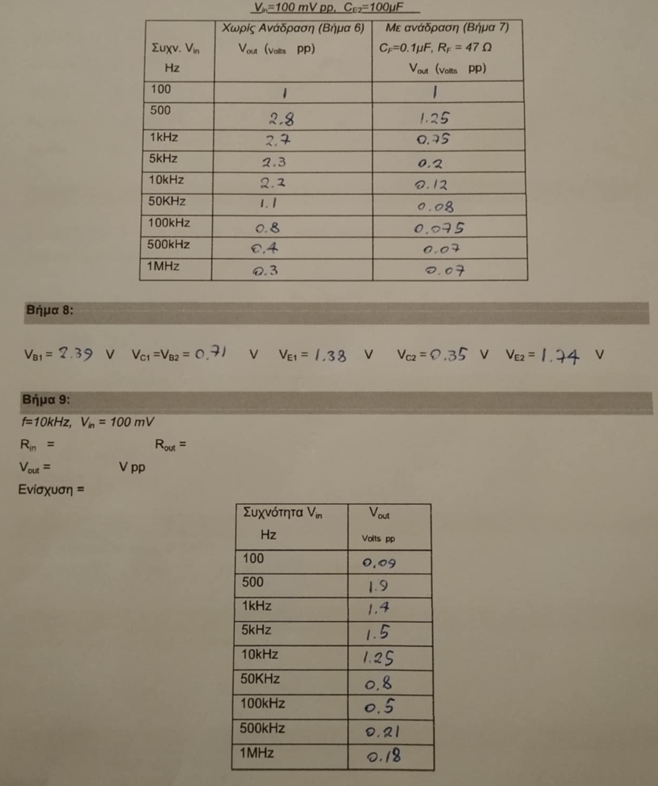
\includegraphics[width=15.0cm]{figures/exercise3experiment2.png}
\caption{Μετρήσεις Εργαστηριακής Άσκησης 3 (δεύτερη σελίδα)}\label{fig:ex3experiment2}
\end{figure}

%%%%%%%%%%%%%%%%%%%%%%%% Exercise 4 %%%%%%%%%%%%%%%%%%%%%%%%
%%%%%%%%%%%%%%%%%%%%%%%%%%%%%%%%%%%%%%%%%%%%%%%%%%%%%%%%%%%%
\chapter{Εργαστηριακή Άσκηση 4}

\section{Βήμα 7}
Η τέταρτη εργαστηριακή άσκηση εξετάζει τρεις διαφορετικές εφαρμογές του τελεστικού ενισχυτή.
\begin{enumerate}
    \item Κύκλωμα Συγκριτή Schmitt Trigger
    \item Κύκλωμα Γεννήτριας Παλμών
    \item Κύκλωμα Ανιχνευτή Διέλευσης από Μηδενική Τάση
\end{enumerate}
Ακολουθούν τα σχετικά σχήματα \ref{fig:ex4circ1} \ref{fig:ex4circ2} \ref{fig:ex4circ3}.
\begin{figure}[H]
    \centering
    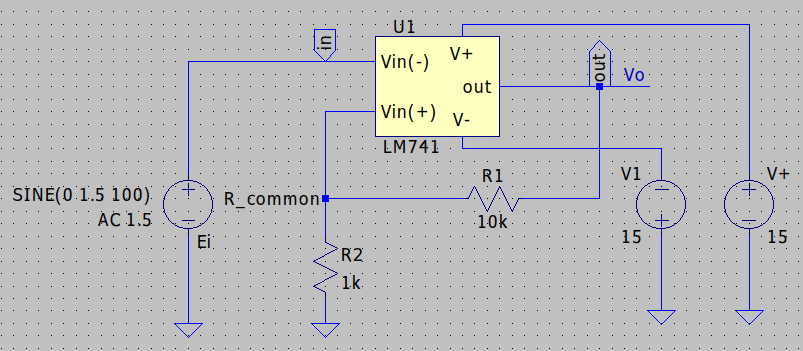
\includegraphics[width=0.8\linewidth]{figures/Exercise4_Schema_4-7.png}
    \caption{Κύκλωμα Συγκριτή Schmitt Trigger}
    \label{fig:ex4circ1}
\end{figure}
\begin{figure}[H]
    \centering
    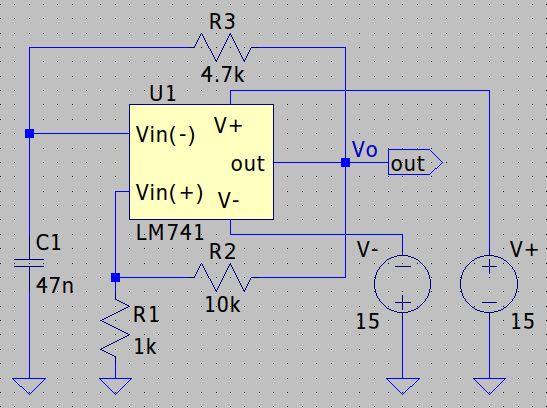
\includegraphics[width=0.8\linewidth]{figures/Exercise4_Schema_4-8.png}
    \caption{Κύκλωμα Γεννήτριας Παλμών}
    \label{fig:ex4circ2}
\end{figure}
\begin{figure}[H]
    \centering
    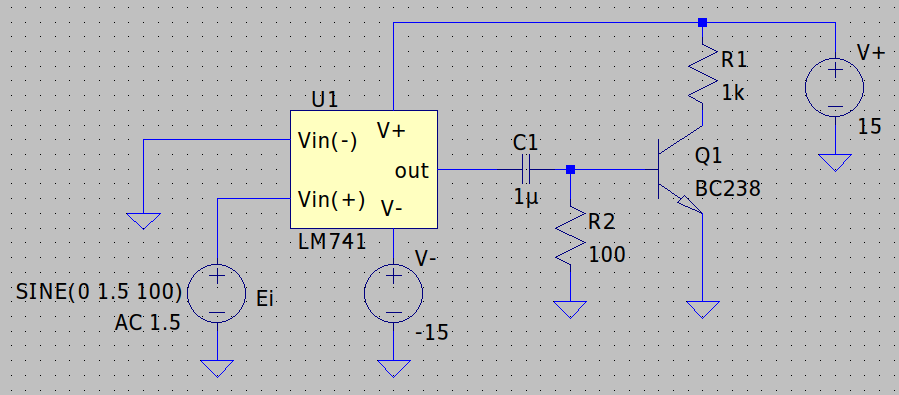
\includegraphics[width=0.8\linewidth]{figures/Exercise4_Schema_4-9.png}
    \caption{Κύκλωμα Ανιχνευτή Διέλευσης από Μηδενική Τάση}
    \label{fig:ex4circ3}
\end{figure}

\section{Βήμα 8}

\paragraph*{} Ξεκινώντας από το κύκλωμα Schmitt Trigger, παρατηρούμε ότι η τάση στο κοινό σημείο των αντιστάσεων $R_1$ και $R_2$ είναι λίγο μικρότερη από το σήμα εισόδου και η έξοδος κυμαίνεται κοντά στα 14$V$ \ref{fig:ex4plot1}.
\begin{figure}[H]
    \centering
    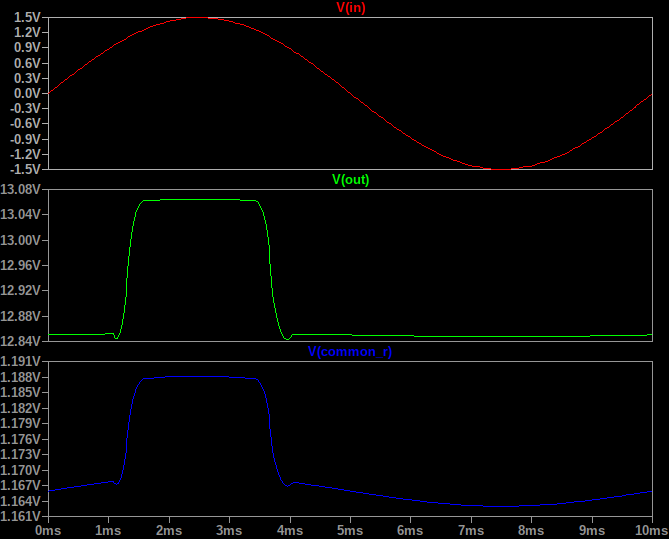
\includegraphics[width=0.8\linewidth]{figures/Exercise4_step2.png}
    \caption{Είσοδος - Έξοδος Schmitt Trigger}
    \label{fig:ex4plot1}
\end{figure}
Τα ευρήματά μας συνάδουν με τα εργαστηριακά μας αποτελέσματα \ref{fig:ex4lab1}.
\begin{figure}[H]
    \centering
    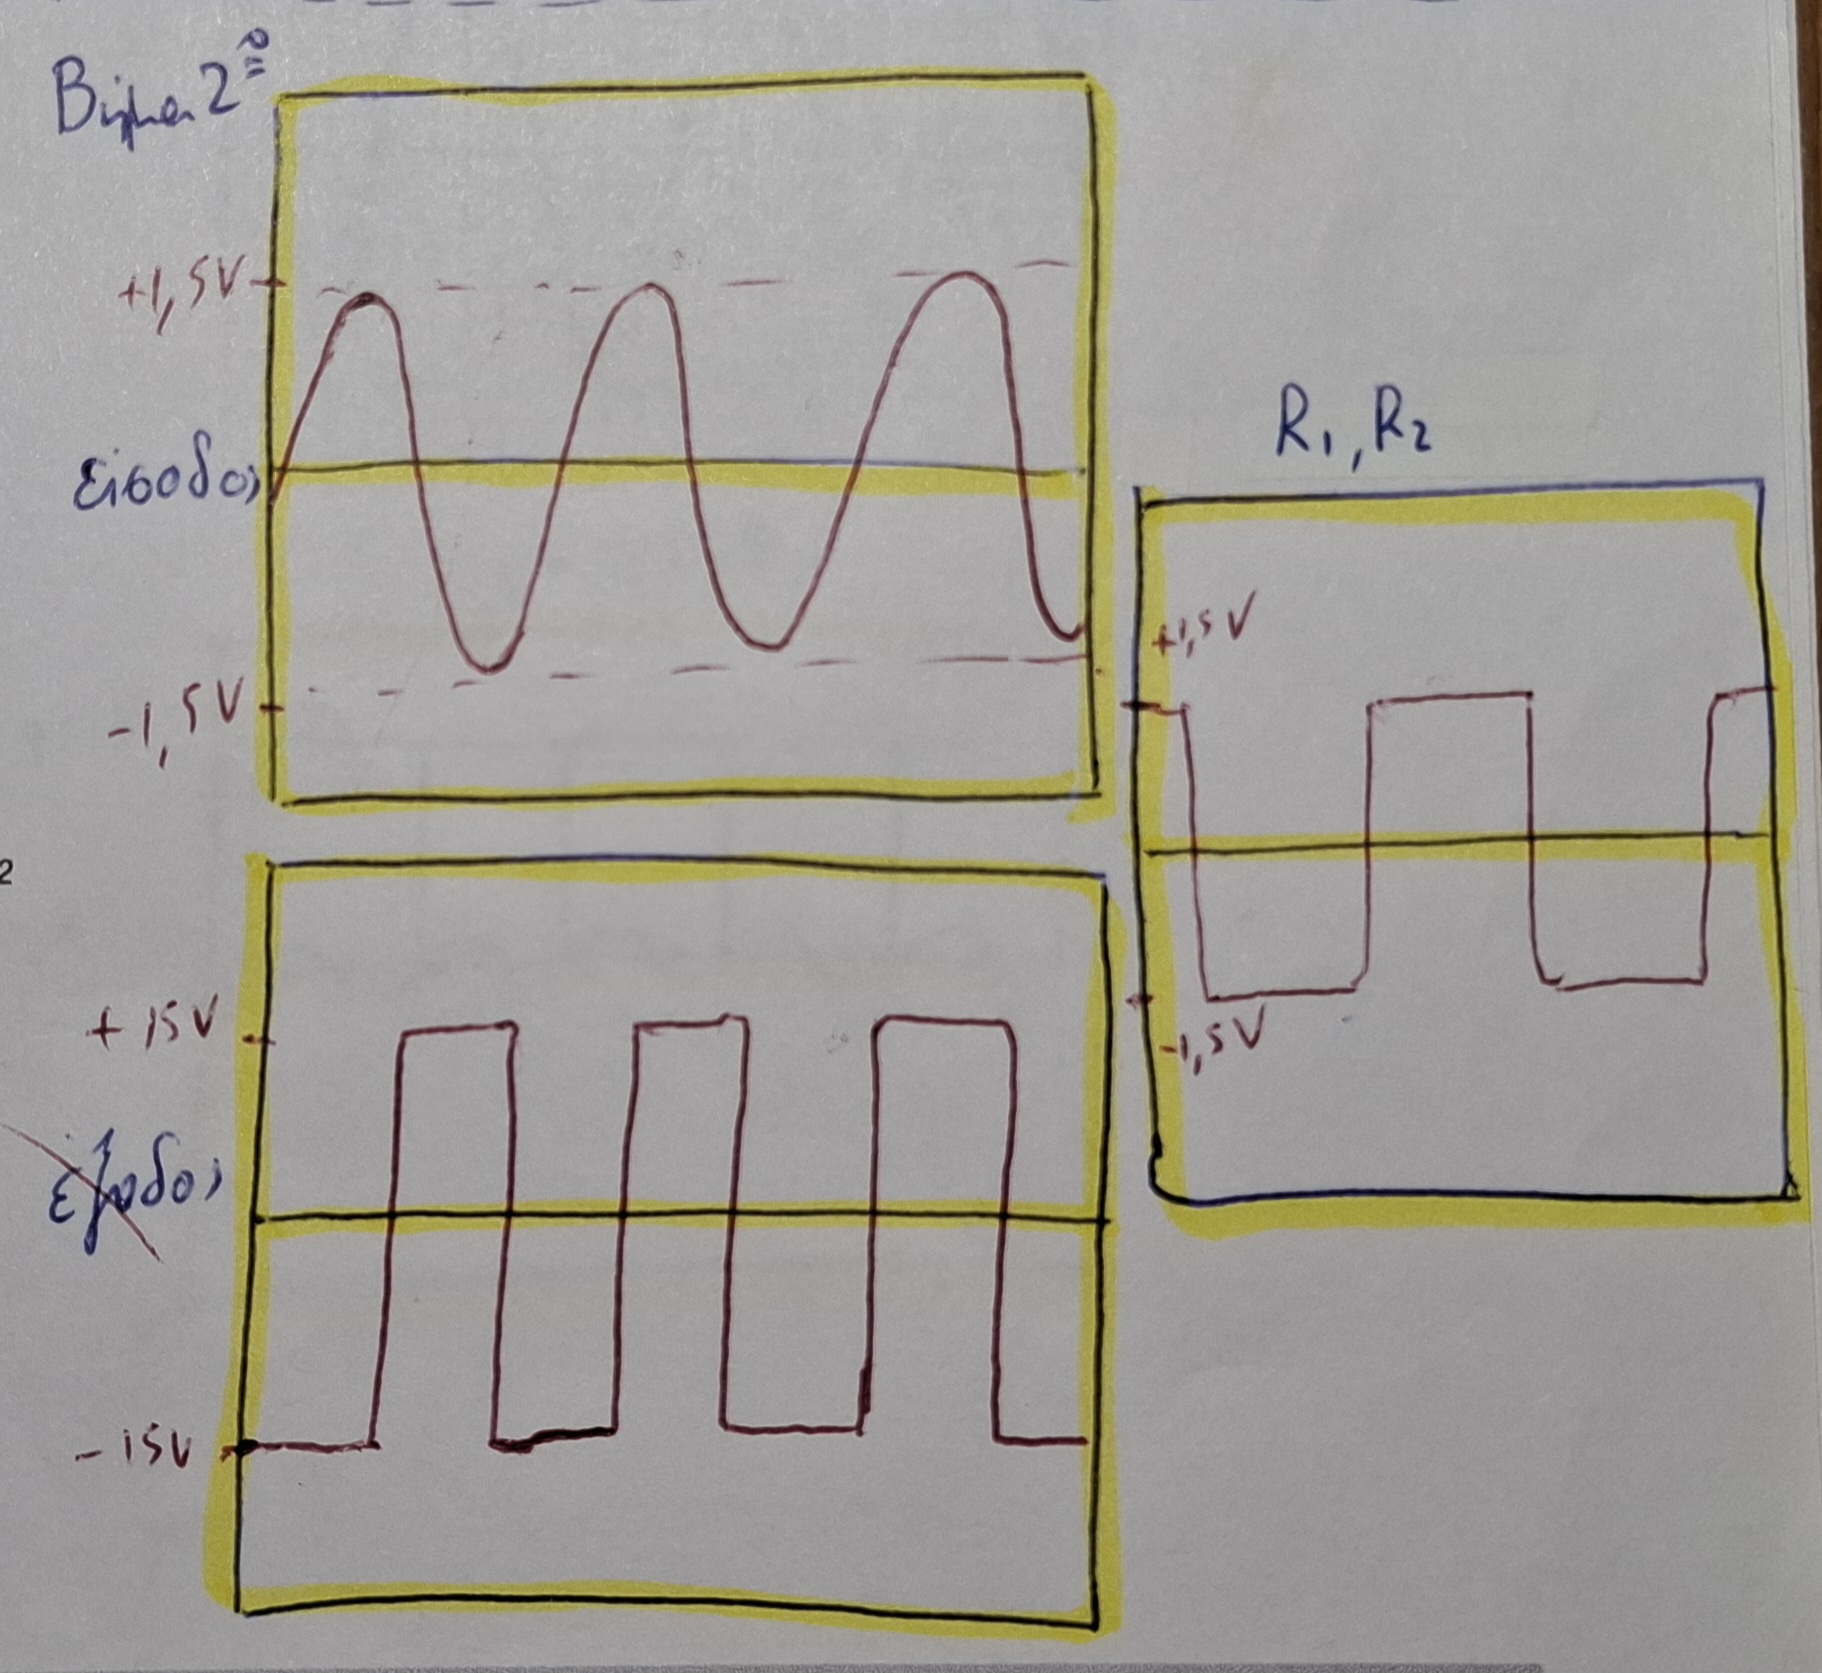
\includegraphics[width=0.7\linewidth]{figures/Exercise4_lab_step2.jpg}
    \caption{Είσοδος - Έξοδος Schmitt Trigger Εργαστήριο}
    \label{fig:ex4lab1}
\end{figure}
Αναλυτικότερα βλέπουμε ότι $V_o=V_{sat}=14V$: 
$$V_{UT}=+14V\frac{R2}{R1+R2}, \quad\quad V_{LT}=-14V\frac{R2}{R1+R2}$$
Αντικαθιστώντας με τις τιμές του κυκλώματος μας έχουμε:
\begin{itemize}
    \item $V_{UT}=+1.2727$
    \item $V_{LT}=-1.2727$
\end{itemize}
Η χρησιμότητά του έγκειται στην προστασία που παρέχει από τον θόρυβο χάρη στην παρουσία υστέρησης $V_{UT} - V_{LT}$.


Στη συνέχεια, το κύκλωμα Γεννήτριας Παλμών παράγει ορθογώνιους παλμούς όπου όταν η έξοδος του
τελεστικού ενισχυτή ισούται με $+V_{sat}$ η τιμή στην οποία φορτίζεται ο πυκνωτής είναι:
$$ V_F = \frac{R_2}{R_1 +R_2} (+V_{sat})$$
Όταν, όμως, η τάση του πυκνωτή φτάσει $-V_{sat}$, εκφορτίζεται λειτουργώντας ως πηγή για τον τελεστικό ενισχυτή \ref{fig:ex4plot2}.
\begin{figure}[H]
    \centering
    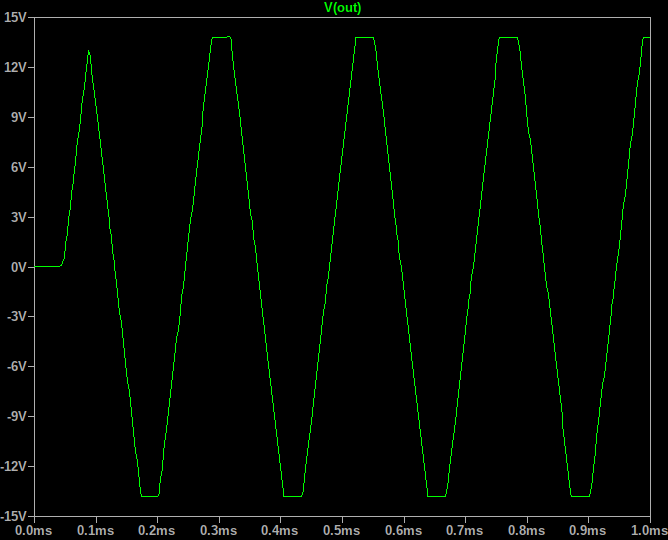
\includegraphics[width=0.8\linewidth]{figures/Exercise4_step5_47n.png}
    \caption{Έξοδος Γεννήτριας Παλμών}
    \label{fig:ex4plot2}
\end{figure}
Στο εργαστήριο τα αποτελέσματά μας ήταν πανομοιότυπα \ref{fig:ex4lab2}.
\begin{figure}[H]
    \centering
    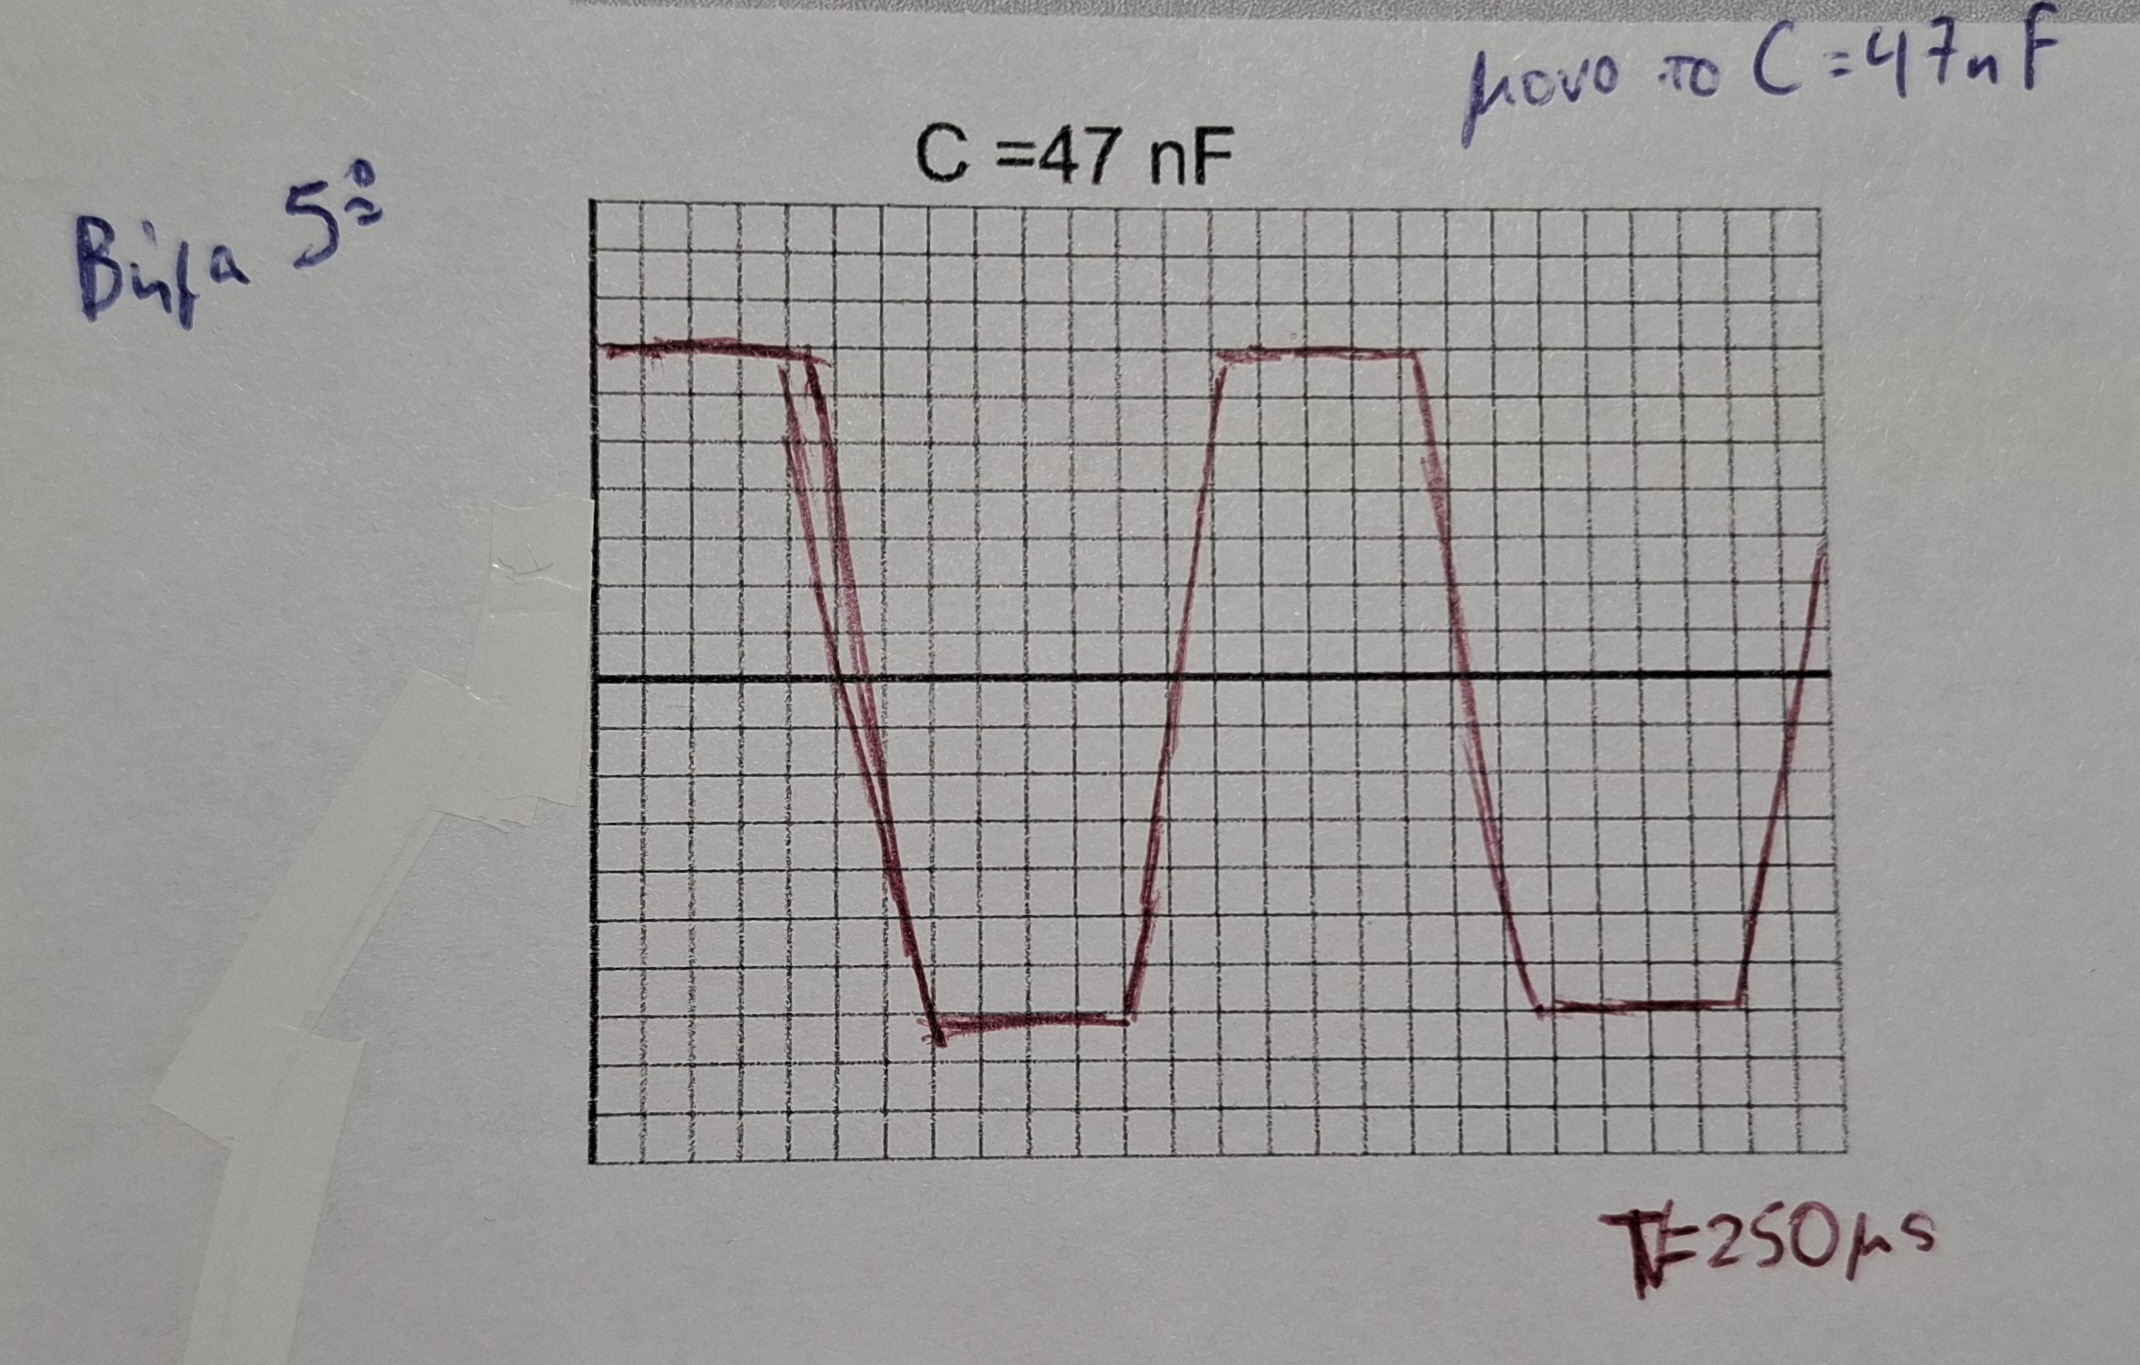
\includegraphics[width=0.8\linewidth]{figures/Exercise4_lab_step5.jpg}
    \caption{Έξοδος Γεννήτριας Παλμών Εργαστήριο}
    \label{fig:ex4lab2}
\end{figure}
Το παραπάνω κύκλωμα χρησιμοποιείται για την παραγωγή σταθερού παλμού ο οποίος εξαρτάται από την σταθερά χρόνου $RC$.


Τέλος, το κύκλωμα Ανιχνευτή Διέλευσης από Μηδενική Τάση παρουσιάζει κορυφή στα $+V_{sat} \approx +14 \ V$ όταν η τάση εισόδου 
είναι θετική. Αλλιώς, όταν η τάση εισόδου είναι αρνητική, η τάση εξόδου οδηγείται στα $-V_{sat} \approx -14 \ V$ \ref{fig:ex4plot3}.
\begin{figure}[H]
    \centering
    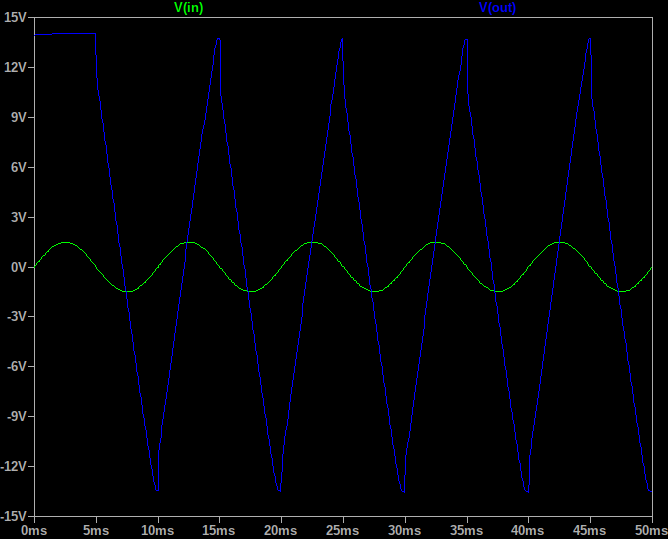
\includegraphics[width=0.8\linewidth]{figures/Exercise4_step6_4dot7u.png}
    \caption{Είσοδος - Έξοδος Ανιχνευτή Διέλευσης από Μηδενική Τάση με C=4.7μF}
    \label{fig:ex4plot3}
\end{figure}
Για μικρότερη τιμή πυκνωτή διακρίνουμε πιο απότομη μετάβαση του τετραγωνικού παλμού καθιστώντας εμφανές το άνω και κάτω πλάτωμα του σήματος εξόδου \ref{fig:ex4plot4}.
\begin{figure}[H]
    \centering
    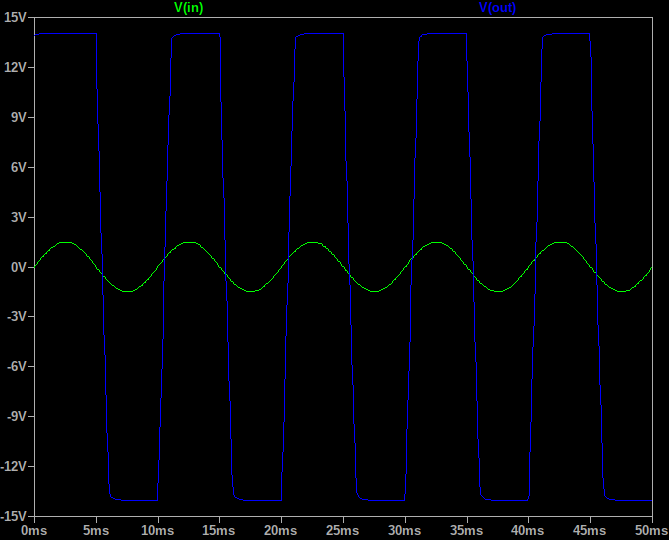
\includegraphics[width=0.8\linewidth]{figures/Exercise4_step6_1u.png}
    \caption{Είσοδος - Έξοδος Ανιχνευτή Διέλευσης από Μηδενική Τάση με C=1μF}
    \label{fig:ex4plot4}
\end{figure}
Εδώ τα αποτελέσματα του εργαστηρίου \ref{fig:ex4lab3} διαφέρουν λίγο από αυτά του SPICE. Τα πειραματικά γραφήματα αδυνατούν να αποτυπώσουν το τριγωνικό σήμα ενώ το τετραγωνικό μένει την περισσότερη ώρα στο πάνω πλάτωμα επιστρέφοντας στιγμιαία στο μηδέν. 
\begin{figure}[H]
    \centering
    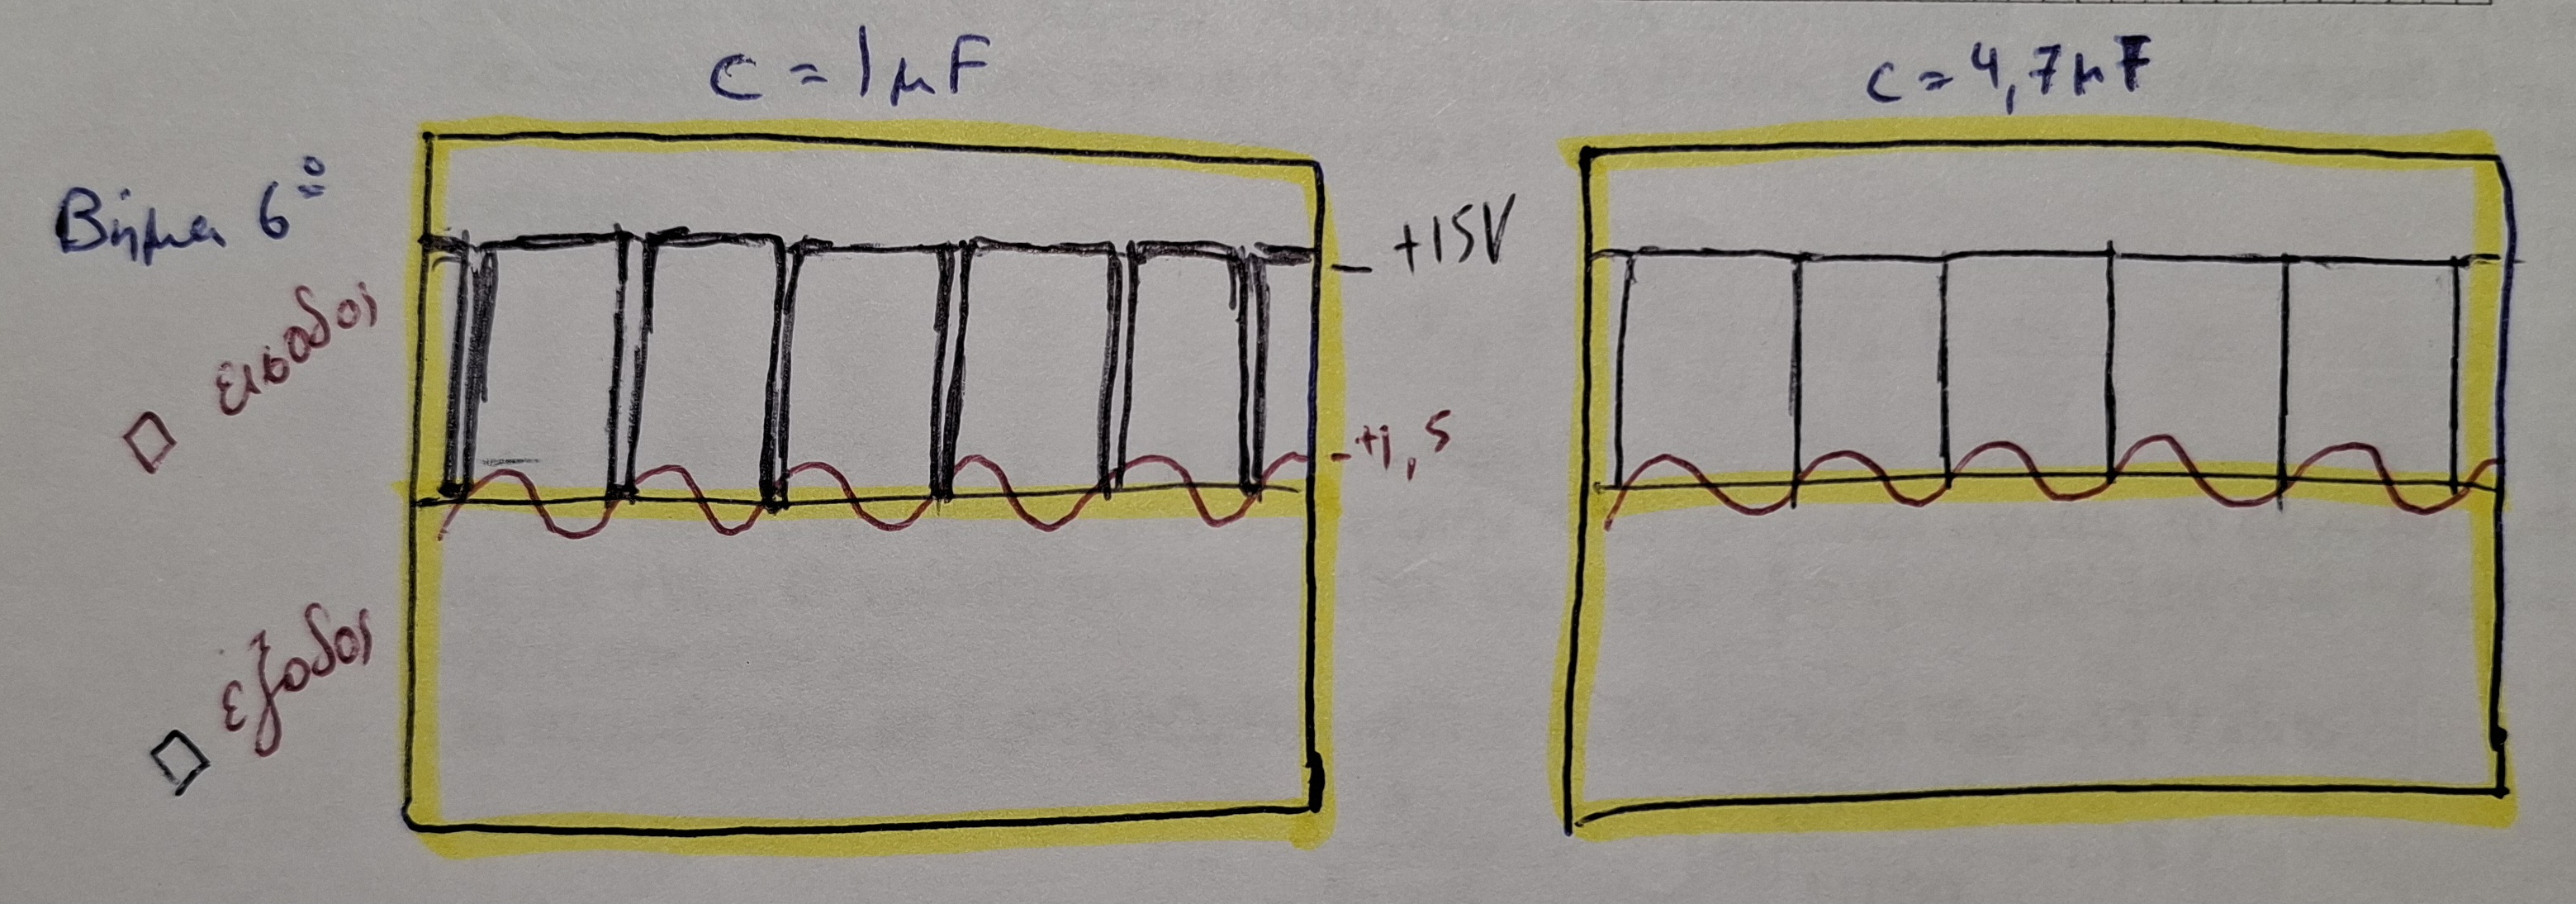
\includegraphics[width=0.8\linewidth]{figures/Exercise4_lab_step6.jpg}
    \caption{Είσοδος - Έξοδος Ανιχνευτή Διέλευσης από Μηδενική Τάση Εργαστήριο}
    \label{fig:ex4lab3}
\end{figure}

%%%%%%%%%%%%%%%%%%%%%%%% Exercise 5 %%%%%%%%%%%%%%%%%%%%%%%%
%%%%%%%%%%%%%%%%%%%%%%%%%%%%%%%%%%%%%%%%%%%%%%%%%%%%%%%%%%%%
\chapter{Εργαστηριακή Άσκηση 5}

\section{Βήμα 13}

\paragraph*{} Υλοποιήθηκε το κύκλωμα του σχήματος 5-4 του φυλλαδίου, όπως φαίνεται στην εικόνα \ref{fig:ex5circuit}.

\begin{figure}[h]
\centerfloat%
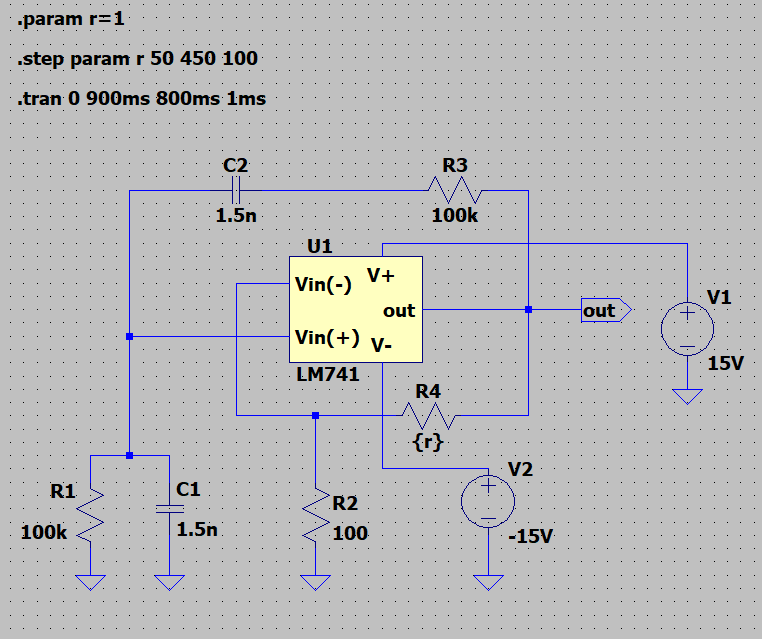
\includegraphics[width=12.0cm]{figures/exercise5circuit1.png}
\caption{Κύκλωμα Ταλαντωτή}\label{fig:ex5circuit}
\end{figure}

Η τάση στον κόμβο εξόδου (out) του τελεστικού ενισχυτή για της διάφορες τιμές της παραμέτρου \(r\) της μεταβλητής αντίστασης \(R_4\) φαίνεται στη σχήμα \ref{fig:ex5plot1}. Παρατηρούμε ότι η μέγιστη τιμή της αντίστασης για την οποία έχουμε ταλαντώσεις σταθερού πλάτους είναι, όπως και στο εργαστηριακό πείραμα, η \(r = 250 \ \Omega\).

\begin{figure}[h]
\centerfloat%
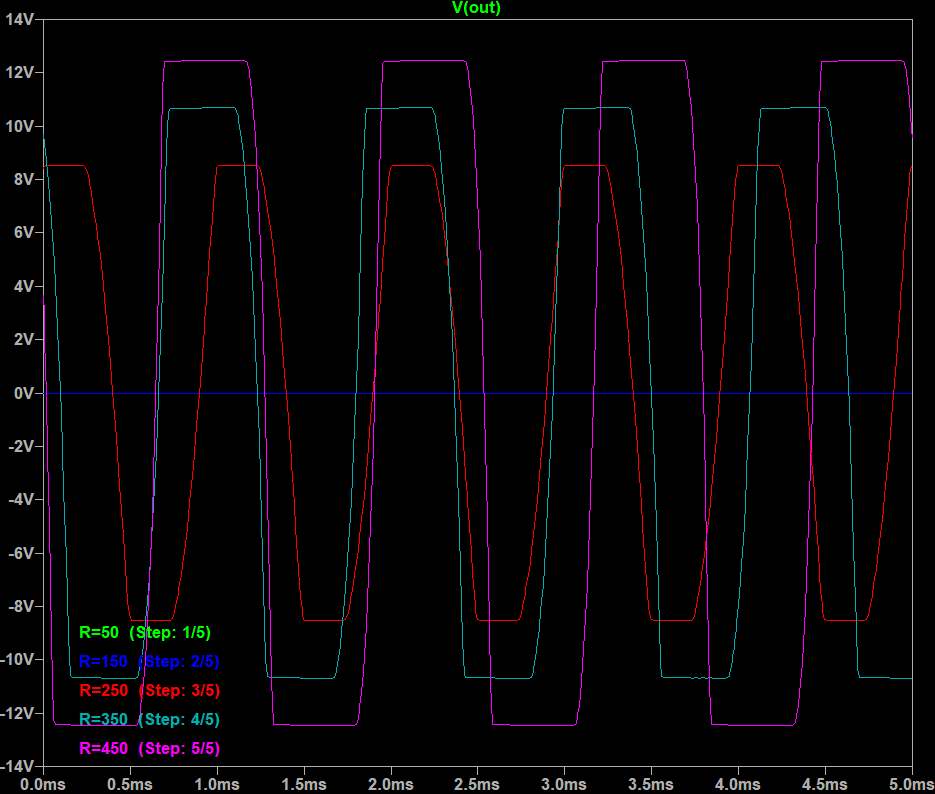
\includegraphics[width=10.0cm]{figures/exercise5plot1.png}
\caption{Έξοδος Ταλαντωτή για Διάφερες Τιμές της Παραμέτρου \(r\)}\label{fig:ex5plot1}
\end{figure}

Σταθεροποιώντας την παράμετρο \(r\) στα \(250 \ \Omega\) παίρνουμε την κυματομορφή του σχήματος \ref{fig:ex5plot2} στην έξοδο του ταλαντωτή.

\begin{figure}[h]
\centerfloat%
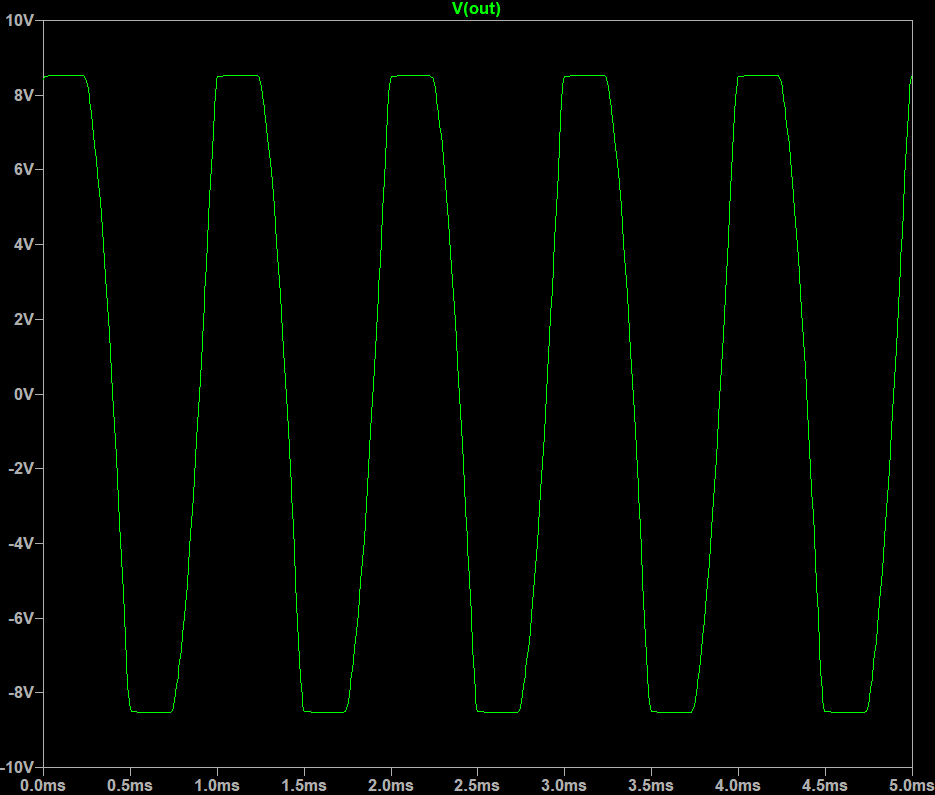
\includegraphics[width=10.0cm]{figures/exercise5plot2.png}
\caption{Έξοδος Ταλαντωτή με Σταθερό \(r\) για \(C = 1.5\ nF\) }\label{fig:ex5plot2}
\end{figure}

Παρατηρούμε ότι η περίοδος της ταλάντωσης είναι \(T = 1 \ ms\) και η αντίστοιχα η συχνότητα είναι \(f = 1 \ kHz\), δεδομένα που συμφωνούν ακριβώς με τις αντίστοιχες τιμές που μετρήθηκαν στο εργαστηριακό πείραμα. Αλλάζοντας τις τιμές των πυκνωτών \(C_1\) και \(C_2\) σε \(47 \ nF\) παίρνουμε στην έξοδο του ταλαντωτή την κυματομορφή του σχήματος \ref{fig:ex5plot3}, για το χρονικό διάστημα \(800 \ ms- 900 \ ms\).

\newpage

\begin{figure}[H]
\centerfloat%
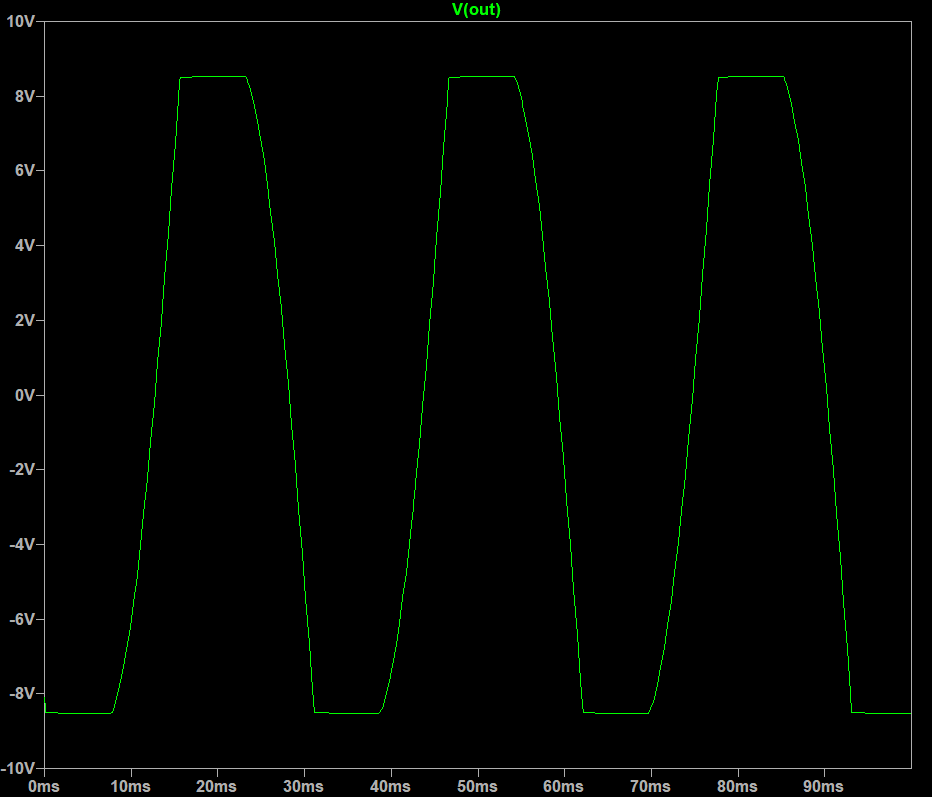
\includegraphics[width=10.0cm]{figures/exercise5plot3.png}
\caption{Έξοδος Ταλαντωτή με Σταθερό \(r\) για \(C = 47\ nF\)}\label{fig:ex5plot3}
\end{figure}



Με την αλλαγή των πυκνωτών, η καινούρια περίοδος είναι \(T = 31.03 \ ms\) και η καινούρια συχνότητα είναι \(f = 32.2 \ Hz\). Οι αντίστοιχες τιμές μετρήθηκαν στο εργαστήριο είναι \(T = 33.3 \ ms\) και \(f = 30 \ Hz\).



Τα γραφήματα που σχεδιάστηκαν στο εργαστηριακό πείραμα, τα οποία είναι πολύ παρόμοια με αυτά που προέκυψαν από τις προσομοιώσεις, φαίνονται στην εικόνα \ref{fig:ex5experiment}.

\begin{figure}[H]
\centerfloat%
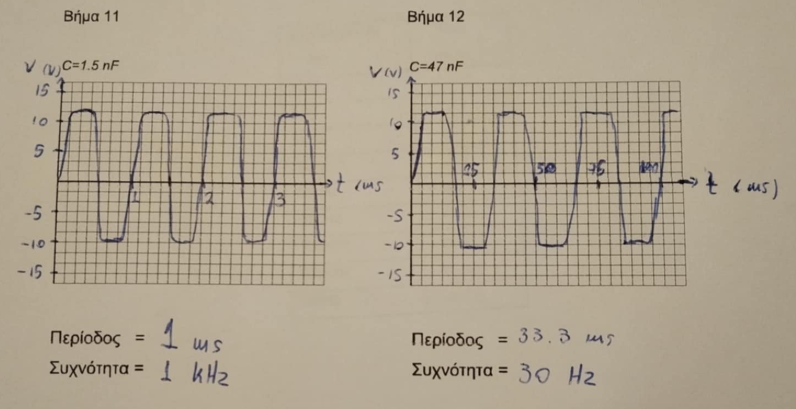
\includegraphics[width=13.0cm]{figures/exercise5experiment.png}
\caption{Μετρήσεις Εργαστηριακής Άσκησης 5}\label{fig:ex5experiment}
\end{figure}

\end{document}

